\BourbakiExerciseGroup

\begin{enumerate}
\def\labelenumi{\arabic{enumi})}
\item
  Let \((x_{i})_{i\in I}\) be a summable family in a complete Hausdorff commutative group \(G\) , and let \(\mathfrak{S}\) be a set of subsets of \(I\) , directed with respect to the relation \(\subset\) and forming a covering of \(I\) . Show that \(\sum_{i\in I}x_{i} = \lim_{J}\sum_{i\in J}x_{i}\) , where the limit is taken with respect to the section filter of \(\mathfrak{S}\) .
\item
  Let G be a complete Hausdorff commutative group such that every neighbourhood of o in G contains an open subgroup of G (this is the case in particular if G is locally compact and totally disconnected; cf.~§ 4, Exercise 18). A family \((x_{t})_{t\in I}\) of points of G is summable if and only if \(\lim x_t = 0\) with respect to the filter of complements of finite subsets of I. Hence show that every convergent series in G is commutatively convergent.
\item
  Let \((x_{i})_{i\in I}\) be a family of points of a Hausdorff commutative group G. For every finite subset H of I, let \(s_{H}\) denote \(\sum_{i\in H}x_{i}\) , and
\end{enumerate}

let A be the set of cluster points of the mapping \(H \rightarrow s_{H}\) with respect to the directed set \(\mathfrak{F}(I)\) . For every finite subset J of I, let \(\Phi(J)\) denote the closure of the set of points \(s_{H}\) , where H runs through the finite subsets of I such that \(H \cap J = \varnothing\) . Show that if \(A \neq \varnothing\) then the set A - A (i.e.~the set of all \(x - x'\) where \(x \in A\) and \(x' \in A\) ) is the same as the set \(B = \bigcap_{J \in \mathfrak{F}(I)} \Phi(J)\) ; and that in any case \(B + B \subset B\) . Deduce that if A is not empty, then B is a closed subgroup of G and that A is a coset of B in G.

\begin{enumerate}
\def\labelenumi{\arabic{enumi})}
\setcounter{enumi}{3}
\item
  With the notation of Exercise 3, take G to be the discrete additive group Z of rational integers and I to be the set N. Give an example of a non-summable sequence \((x_{n})\) for which the set A consists of the single point o (choose the \(x_{n}\) so that every finite partial sum, all of whose terms have indices \(\geqslant m\) , is an integral multiple of m).
\item
  Let \((x_{n})\) be a sequence of points of a Hausdorff commutative group. If, for every infinite subset I of N, the series defined by the sequence \((x_{n})_{n\in I}\) is convergent, then the sequence \((x_{n})\) is summable (argue by reductio ad absurdum as in the proof of Proposition 9).
\end{enumerate}

¶ 6) a) Let \(\sigma\) be a permutation of \(\mathbf{N}\) and let \(\varphi(n)\) be the smallest number of intervals of \(\mathbf{N}\) whose union is \(\sigma([0, n])\) . Suppose that \(\varphi(n)\) is bounded as \(n\) runs through \(\mathbf{N}\) . Then if \((u_n)\) is any convergent series whose terms belong to a Hausdorff commutative group \(\mathbf{G}\) , the series \((u_{\sigma(n)})\) is convergent and has the same sum as \((u_n)\) .

* b) Suppose that \(\varphi(n)\) is not bounded in N. Construct a series \((u_n)\) whose terms belong to the additive group R and which converges in R but is such that the series \((u_{\sigma(n)})\) does not converge. {[}Consider a strictly increasing sequence \((m_k)\) of integers, defined by induction on \(k\) , satisfying the following conditions: (i) if \([0, n_k]\) is the largest interval of N with left-hand extremity o which is contained in \(\sigma([0, m_k])\) , then

\[
\sigma ([ 0, m _ {k} ]) \subset [ 0, n _ {k + 1} ];
\]

\begin{enumerate}
\def\labelenumi{(\roman{enumi})}
\setcounter{enumi}{1}
\tightlist
\item
  \(\varphi(m_k) \geqslant k + 1\) . Then define \(u_n\) appropriately for \(n_k < n < n_{k+1}]\) . Generalize to the case of a complete Hausdorff commutative group G which is generated by every neighbourhood of o. *
\end{enumerate}

\begin{enumerate}
\def\labelenumi{\arabic{enumi})}
\setcounter{enumi}{6}
\tightlist
\item
  Let \((x_{mn})\) be a double sequence of points of a Hausdorff commutative group \(\mathbf{G}\) , satisfying the following conditions:
\end{enumerate}

\begin{enumerate}
\def\labelenumi{(\alph{enumi})}
\item
  The series defined by the sequence \((x_{mn})_{n\in \mathbb{N}}\) is convergent for each \(m\geqslant 0\) ; let \(y_{m}\) be its sum.
\item
  If we put \(r_{mn} = \sum_{p=n}^{\infty} x_{mp}\) , then the series defined by the sequence \((r_{mn})_{m \in \mathbb{N}}\) is convergent for each \(n \geqslant 0\) ; let \(t_n\) be its sum.
\end{enumerate}

Show that for each \(n \geqslant 0\) the series defined by the sequence \((x_{mn})_{m \in \mathbb{N}}\) is convergent, and let \(z_{n}\) be its sum. The series whose general term is \(y_{m}\) has the same sum as the series whose general term is \(z_{n}\) if and only if \(t_{n}\) tends to 0 as n tends to infinity.

\BourbakiExerciseGroup

\begin{enumerate}
\def\labelenumi{\arabic{enumi})}
\item
  In a Hausdorff topological ring A, the commutant of every subset of A (and in particular the centre of A) is closed, and so is the left (resp. right) annihilator of every subset of A.
\item
  \begin{enumerate}
  \def\labelenumii{\alph{enumii})}
  \tightlist
  \item
    Let \(\mathfrak{a}\) be a discrete left ideal in a topological ring A. Show that, for every \(x \in \mathfrak{a}\) , the left annihilator of \(x\) in A is open. Hence show that if A is a non-discrete ring with no zero-divisors, it contains no discrete (left or right) ideal other than \(\{\mathbf{o}\}\) .
  \end{enumerate}
\end{enumerate}

\begin{enumerate}
\def\labelenumi{\alph{enumi})}
\setcounter{enumi}{1}
\tightlist
\item
  Let A be a locally connected topological ring, and let \(\mathfrak{a}\) be a totally disconnected left ideal of A. Show that, for each \(x \in \mathfrak{a}\) , the left annihilator of \(x\) in A is open. Hence show that if A has no zero-divisors it contains no totally disconnected (left or right) ideal other than \(\{0\}\) .
\end{enumerate}

\begin{enumerate}
\def\labelenumi{\arabic{enumi})}
\setcounter{enumi}{2}
\item
  The connected component of o in a topological ring A is a two-sided ideal. Deduce that if A is quasi-simple and is not connected (in particular, if A is a non-connected topological division ring) then A is totally disconnected.
\item
  Let \((x_{i})\) be a summable family in a Hausdorff topological ring A, and let \(s\) be its sum. Then for each \(a \in A\) the family \((ax_{i})\) {[}resp. \((x_{i}a)]\) is summable and its sum is as (resp. sa). If \((x_{\lambda})\) and \((y_{\mu})\) are two summable families in A such that the family \((x_{\lambda}y_{\mu})\) is summable, then \(\sum_{\lambda,\mu} x_{\lambda} y_{\mu} = \left( \sum_{\lambda} x_{\lambda} \right) \left( \sum_{\mu} y_{\mu} \right)\) . If moreover A is complete and if one of the \(x_{\lambda}\) is a unit, then the summability of the family \((x_{\lambda}y_{\mu})\) implies the summability of \((y_{\mu})\) .
\item
  A rectangle is a subset of \(N \times N\) which is the product of two intervals of N. Given a finite subset E of \(N \times N\) , let \(\varphi(E)\) be the smallest number of mutually disjoint rectangles whose union is E. Let \((E_n)\) be an increasing sequence of finite subsets of \(N \times N\) which cover \(N \times N\) and are such that the sequence \((\varphi(E_n))\) is bounded. If \((x_n), (y_n)\) are two convergent series whose terms belong to a Hausdorff topological ring A, then we have
\end{enumerate}

\[
\lim _ {n \rightarrow \infty} \sum_ {(h, k) \in \mathrm{E} _ {n}} x _ {h} y _ {k} = \left(\underset {n = 0} {\overset {\infty} {\sum}} x _ {n}\right)\left(\underset {n = 0} {\overset {\infty} {\sum}} y _ {n}\right).
\]

Construct an example of a sequence \((\mathbf{E}_{n})\) satisfying the conditions above and such that \(E_{n+1} - E_{n}\) contains only one element for each n.

\begin{enumerate}
\def\labelenumi{\arabic{enumi})}
\setcounter{enumi}{5}
\item
  Let A be a topological ring with an identity element and let \(a, b\) be two two-sided ideals of A such that \(a + b = A\) and \(a \cap b = \{0\}\) . Show that the topological ring A is isomorphic to the product of the topological rings a and b.
\item
  Let A be a topological ring with no identity element, and let B be the ring obtained by adjoining an identity element to A show that the topology on B which is the product of the topology of A and the discrete topology on Z is compatible with the ring structure of B, and induces the given topology on A (a two-sided ideal of B).
\item
  Let \(\mathbf{A}\) be a topological ring with an identity element.
\end{enumerate}

\begin{enumerate}
\def\labelenumi{\alph{enumi})}
\item
  The set A* of units of A is open in A if and only if there is a neighbourhood V of 1 all of whose elements are units in A.
\item
  If A* is open in A then every maximal (left or right) ideal of A is closed, and the radical of A is closed. If A has no closed left ideals other than \(\{o\}\) and A, then A is a division ring.
\item
  Let A be the subring of the topological field Q consisting of all rational numbers \(k/2^{n}\) ( \(k \in Z, n \in N\) ). Show that A contains no closed ideal other than \(\{0\}\) and A, but is not a field.
\end{enumerate}

\begin{enumerate}
\def\labelenumi{\arabic{enumi})}
\setcounter{enumi}{8}
\tightlist
\item
  \begin{enumerate}
  \def\labelenumii{\alph{enumii})}
  \tightlist
  \item
    An element \(x\) (resp. an ideal \(\mathfrak{a}\) ) of a topological ring \(\mathbf{A}\) is said to be topologically nilpotent if the sequence \((x^n)_{n\geqslant 1}\) converges to o {[}resp. if the filter base formed by the \(\mathfrak{a}^n\) ( \(n\geqslant 1\) ) converges to o). Every element of a topologically nilpotent ideal is topologically nilpotent.
  \end{enumerate}
\end{enumerate}

\begin{enumerate}
\def\labelenumi{\alph{enumi})}
\setcounter{enumi}{1}
\item
  Suppose that A has an identity element and that \(A^{*}\) is open in A. Show that if x is any topologically nilpotent element of A, then 1 - x is a unit (observe that \(1 - x^{n}\) is a unit for sufficiently large n). Hence show that if all the elements of a (left or right) ideal a are topologically nilpotent, then a is contained in the radical of A.
\item
  Suppose that A is complete and has an identity element, and that there exists a fundamental system of neighbourhoods of o which are subgroups of the additive group of A. Show that if x is topologically nilpotent, then 1 - x is a unit in A.
\end{enumerate}

\(d)\) Under the hypotheses of \(c\) ), show that if \(y \in A\) is topologically nilpotent, then the equation \(x^{2} + x = y\) has a root \(x \in A\) , and that \(x\) is topologically nilpotent.

¶ 10) a) Let B be a ring with an identity element, let E be a free B-module \(\mathbf{B}_{d}^{(I)}\) , and let A be the ring \(\mathcal{L}(\mathbf{E})\) of endomorphisms of E. For every finite subset F of E, let \(V_{F}\) be the set of all \(u \in A\) such that \(u(x) = 0\) for all \(x \in F\) . Show that the \(V_{F}\) from a fundamental system of neighbourhoods of o for a Hausdorff topology on A, which is compatible with the ring structure of A, and with respect to which A is totally disconnected.

\begin{enumerate}
\def\labelenumi{\alph{enumi})}
\setcounter{enumi}{1}
\tightlist
\item
  Take I = N and take B to be a commutative ring which has no zero-divisors but whose radical R is not \(\{0\}\) . Show that the radical of A is not closed. {[}Let \((e_{n})\) be the canonical basis of E. Remark on the one hand that each \(u \in A\) , such that \(u(e_{n}) = 0\) for all but a finite number of indices and such that \(u(E) \subset \Re \cdot E\) , belongs to the radical of A; consider on the other hand the element \(u_{0}\) of A such that \(u_{0}(e_{n}) = e_{n} + te_{n+1}\) with \(t \neq 0\) in R, for each n{]}.
\end{enumerate}

¶ 11) a) A topological ring with an identity element is said to be a Gelfand ring if A* is open in A and if the topology induced on A* by the topology of A is compatible with the multiplicative group structure of A*. Every Hausdorff topological division ring is a Gelfand ring {[}cf.~Exercise 20 e){]}.

\begin{enumerate}
\def\labelenumi{\alph{enumi})}
\setcounter{enumi}{1}
\tightlist
\item
  Show that if A is a Gelfand ring then so is every matrix ring \(\mathbf{M}_{n}(\mathbf{A})\) endowed with the product topology (on \(A^{n^{2}}\) ). (Proof by induction on n).
\end{enumerate}

\begin{enumerate}
\def\labelenumi{\arabic{enumi})}
\setcounter{enumi}{11}
\tightlist
\item
  A subset M of a topological ring is said to be right bounded (resp. left bounded) if, for each neighbourhood U of o in A, there is a neighbourhood V of o such that VM⊂U (resp. MV⊂U); M is bounded if it is both left and right bounded. The topology of A is said to be locally bounded (and A is said to be a locally bounded topological ring) if there is a bounded neighbourhood of o in A.
\end{enumerate}

\begin{enumerate}
\def\labelenumi{\alph{enumi})}
\item
  Every topological ring which has a fundamental system of neighbourhoods of o consisting of right ideals is right bounded. Show that if I is infinite and B is a division ring in Exercise 10 a), then the ring A is left bounded, but there is no right bounded neighbourhood of o in A.
\item
  If a topological ring A is right bounded (resp. bounded) and has a fundamental system of neighbourhoods of o which are subgroups of the additive group of A, then it has a fundamental system of neighbourhoods of o which are right (resp. two-sided) ideals.
\item
  Every finite union of bounded sets is bounded; the closure of a bounded set is bounded; if M and N are bounded, then so are \(M + N\) and MN.
\item
  Every precompact set in a topological ring \(\mathbf{A}\) is bounded.
\item
  If M and N are two bounded subsets of A, show that the mapping \((x, y) \to xy\) elements of \(M \times N\) into A is uniformly continuous.
\item
  Let A be a Hausdorff topological ring which has an identity element. Show that if \((x_{n})\) is a sequence of units which tends to o in A, then the set of elements \(x_{n}^{-1}\) is neither left nor right bounded.
\item
  If A is a bounded ring with an identity element, show that the mapping \(x \rightarrow x^{-1}\) is uniformly continuous on the set A* of units of A. h) Show that if A is a complete Hausdorff bounded ring with an identity element, then the set A* of units and the radical of A are closed {[}use g){]}.
\item
  A subset of a product \(\prod_{t} A_{t}\) of topological rings is bounded if and only if all its projections are bounded.
\item
  Every subring of a locally bounded ring and every product of locally bounded rings are locally bounded rings.
\item
  The completion of a locally bounded Hausdorff ring is locally bounded.
\end{enumerate}

\begin{enumerate}
\def\labelenumi{\arabic{enumi})}
\setcounter{enumi}{12}
\tightlist
\item
  Let A be a bounded topological ring (Exercise 12) which has an identity element and is such that the set A* of units of A is open in A. Show that the radical of A is open. Hence if A is without radical, it is discrete; in particular, a bounded Hausdorff topological division ring is discrete. A compact ring A without radical, which has an identity element and in which A* is open, is finite; in particular, a compact topological division ring is finite.
\end{enumerate}

¶ 14) Let A be a compact ring with an identity element, totally disconnected (*) and without radical. Then A is isomorphic to the product of a family of finite simple rings. {[}Show first that A has a fundamental system of neighbourhoods of o which are two-sided ideals, using Exercise 12 b) of § 6 and Proposition 14 of § 4. Hence show that there is a maximal set \(\Phi\) of two-sided ideals of A such that (i) every two-sided ideal \(\mathfrak{M} \in \Phi\) is a maximal open two-sided ideal of A; (ii) no ideal \(\mathfrak{M} \in \Phi\) contains a finite intersection of ideals of \(\Phi\) other than \(\mathfrak{M}\). Show then that A is isomorphic to the product of the rings \(A/\mathfrak{M}\) as \(\mathfrak{M}\) runs through \(\Phi\); prove first that the intersection of all the \(\mathfrak{M} \in \Phi\) consists only of the zero element of A by using Exercise 9 b){]}.
(*) It can be shown that a compact ring with an identity element is necessarily totally disconnected.

\begin{enumerate}
\def\labelenumi{\arabic{enumi})}
\setcounter{enumi}{14}
\item
  Let A be a totally disconnected compact ring with an identity element. Show that the radical \(\Re\) of A is topologically nilpotent {[}Exercise 9 a); use Exercise 12 b) of § 6 and Proposition 14 of § 4{]}. Hence show that \(\Re\) is the set of all \(x \in A\) such that \(ax\) is topologically nilpotent for all \(a \in A\) {[}cf.~Exercise 9 c){]}.
\item
  Show that on a ring A (resp. a division ring K), the least upper bound \(\mathcal{C}\) of a family \((\mathcal{T}_i)\) of topologies compatible with the ring structure of A (resp. the division ring structure of K) is compatible with this structure. A set M which is left (resp. right) bounded for each of the topologies \(\mathcal{T}_i\) is also left (resp. right) bounded for \(\mathcal{C}\) .
\item
  If K is a Hausdorff topological division ring and is not discrete, then neither of the multiplicative uniformities on K is comparable with the uniformity induced on \(K^{*}\) by the additive uniformity of K (cf.~Exercise 13).
\item
  Let K be a Hausdorff topological division ring, let A be a closed subset of K and let B be a compact subset of K such that \(o \notin B\) . Show that AB and BA are closed in K (cf.~§ 4, no. 1, Proposition 1, Corollary 1). * In the field R of real numbers, give an example where A is closed, and B is compact, \(o \in B\) and AB is not closed. *
\item
  \begin{enumerate}
  \def\labelenumii{\alph{enumii})}
  \tightlist
  \item
    Let K be a division ring endowed with a Hausdorff topology \(\mathcal{G}\) compatible with the ring structure of K. Show that there is a neighbourhood V of o in K such that \((\mathbb{CV}) \cup (\mathbb{CV})^{-1} = \mathbf{K}^*\) {[}this is equivalent to \(\mathbf{V} \cap (\mathbf{V} \cap \mathbf{K}^*)^{-1} = \emptyset\) {]}.
  \end{enumerate}
\end{enumerate}

\begin{enumerate}
\def\labelenumi{\alph{enumi})}
\setcounter{enumi}{1}
\tightlist
\item
  Suppose moreover that \(\mathfrak{C}\) is not discrete. Show that if \(\mathbf{U}\) is any neighbourhood of \(o\) in \(\mathbf{K}\) and if \(\mathbf{U}^*\) denotes \(\mathbf{U} \cap \mathbf{K}^*\) , then
\end{enumerate}

\[
\mathbf {U} ^ {*} (\mathbf {U} ^ {*}) ^ {- 1} = \mathbf {K} ^ {*}.
\]

¶ 20) a) Let K be a division ring endowed with a non-discrete Hausdorff topology \(\mathfrak{C}\) compatible with the ring structure of K. A subset M of K is right (resp. left) bounded if and only if, for each neighbourhood U of o there exists \(a \in \mathbf{K}^*\) such that \(a\mathbf{M} \subset \mathbf{U}\) (resp. Ma \(\subset\) U); M is then right (resp. left) bounded for every Hausdorff topology \(\mathfrak{C}'\) which is coarser than \(\mathfrak{C}\) and is compatible with the ring structure of K.

\begin{enumerate}
\def\labelenumi{\alph{enumi})}
\setcounter{enumi}{1}
\item
  If \(\mathfrak{G}\) is locally bounded (Exercise 12) and if U is a bounded neighbourhood of o with respect to \(\mathfrak{G}\) , then the sets \(x\mathrm{U}\) (resp. \(\mathrm{U}x\) ) form a fundamental system of neighbourhoods of o (with respect to \(\mathfrak{G}\) ) as x runs through \(\mathbf{K}^*\) . Every point of K has a countable fundamental system of neighbourhoods of o with respect to \(\mathfrak{G}\) if and only if there is a sequence \((a_n)\) of points of K which has o as a cluster point.
\item
  The least upper bound of any finite family of locally bounded topologies on K (compatible with the ring structure of K) is locally bounded. Conversely, if the least upper bound \(\mathcal{G}\) of a family \((\mathfrak{T}_i)\) of locally bounded topologies on K is locally bounded, then \(\mathcal{G}\) is the least upper bound of a finite subfamily of \((\mathfrak{T}_i)\) . (Remark that if U is a neighbourhood of o which is bounded with respect to \(\mathcal{G}\) , then there is a finite system of indices \((\iota_k)\) and for each \(k\) a neighbourhood \(\mathrm{V}_k\) of o, bounded with respect to \(\mathcal{G}_{\iota_k}\) , such that \(\bigcap \mathrm{V}_k \subset \mathrm{U}\) ; on the other hand, there exists \(a_k \in \mathrm{K}^*\) such that \(\mathrm{U} \subset a_k \mathrm{V}_{k'}\) .)
\item
  A subset F of a division ring K is said to be a quasi-ring if: (i) \(F \neq K\) , \(o \in F\) , \(1 \in F\) , \(-F = F\) , \(FF \subset F\) ; (ii) there is an element \(c \in F^{*} = F \cap K^{*}\) such that \(c(F + F) \subset F\) ; and (iii) for each \(x \in F\) , there exists \(y \in F\) such that \(yF \subset Fx\) and \(Fy \subset xF\) . Show that if G is a non-discrete Hausdorff topology which is locally bounded and compatible with the ring structure of K, then every symmetric bounded neighbourhood U of o (with respect to G), such that \(UU \subset U\) and \(1 \in U\) , is a quasi-ring, and that \(U^{*}(U^{*})^{-1} = K^{*}\) {[}Exercise 19 b){]}. If V is any symmetric bounded neighbourhood of o with respect to G, then the set U of elements \(x \in K\) such that \(xV \subset V\) (or \(Vx \subset V\) ) is a symmetric bounded neighbourhood of o with respect to G such that \(UU \subset U\) and \(1 \in U\) , and hence is a quasi-ring.
\item
  Conversely, let F be a quasi-ring in K such that \(\mathrm{F}^{*}(\mathrm{F}^{*})^{-1} = \mathrm{K}^{*}\) . Show that there is a Hausdorff topology G which is not discrete and is compatible with the ring structure of K, such that F is a bounded neighbourhood of o with respect to G. In particular we may take F to be any subring A of K such that K is the division ring of right fractions of A. In particular, if K = Q and F = Z, the corresponding topology G on K is not compatible with the field structure of K.
\end{enumerate}

¶ 21) a) Let \(\mathfrak{C}\) be a locally bounded Hausdorff topology on a division ring K, with respect to which K is connected. Show that there are non-zero topologically nilpotent elements {[}Exercise 9 a){]} in K. (If U is a symmetric bounded neighbourhood of o, and t is a non-zero element of K such that \(\mathrm{U}t + t\mathrm{U} \subset \mathrm{U}\) , show that K is the union of the sets \(\mathrm{U}t^{-n}\) , by using Proposition 6 of § 2, no. 2).

\begin{enumerate}
\def\labelenumi{\alph{enumi})}
\setcounter{enumi}{1}
\tightlist
\item
  Let \(\mathfrak{G}\) be a locally bounded Hausdorff topology on K, with respect to which K has non-zero topologically nilpotent elements. Show that there is a neighbourhood U of o such that, for each neighbourhood V of o, there is an integer \(n_0\) such that \(\mathrm{U}^n\subset \mathrm{V}\) whenever \(n\geqslant n_0\) ; this implies that all the elements of U are topologically nilpotent and that every point of K has a countable fundamental system of neighbourhoods with respect to \(\mathfrak{G}\) . (Let \(t\neq 0\) be topologically nilpotent and let W be a bounded neighbourhood of o; take U to be a bounded neighbourhood of o such that \(\mathrm{UW}\subset \mathrm{Wt}\) .) The set T of topologically nilpotent elements of K is therefore a neighbourhood of o with respect to \(\mathfrak{G}\) .
\end{enumerate}

¶ 22) In a division ring K endowed with a Hausdorff topology \(\mathfrak{G}\) compatible with the ring structure of K, a set R containing o is said to be retrobounded if \((\mathbb{C}R)^{-1}\) is bounded. \(\mathfrak{G}\) is said to be locally retrobounded if there is a fundamental system of retrobounded neighbourhoods of o in K with respect to \(\mathfrak{G}\) .

\begin{enumerate}
\def\labelenumi{\alph{enumi})}
\item
  A locally retrobounded topology T is locally bounded, and is a minimal element in the set of all Hausdorff topologies compatible with the ring structure of K; also C is compatible with the division ring structure of K {[}use Exercise 19 a){]}.
\item
  Suppose from now on, in this exercise, that \(\mathcal{G}\) is a locally retrobounded topology on K. Show that, for every neighbourhood V of o in K, \(x \to x^{-1}\) is uniformly continuous on \(\mathbb{C}\mathrm{V}\) . Hence show that the completion \(\hat{\mathbf{K}}\) of K is a topological division ring whose topology is locally retrobounded.
\item
  Every neighbourhood of o in K (with respect to \(\mathfrak{G}\) ) contains a neighbourhood V of o such that \(\mathbf{E}(\mathbf{V}) = (\mathbb{C}\mathbf{V}) \cap (\mathbb{C}\mathbf{V})^{-1}\) is not empty. Show that the three uniformities on \(\mathbf{E}(\mathbf{V})\) , induced by the additive uniformity and the two multiplicative uniformities on K, coincide. Deduce that, if K is complete, then \(\mathbf{K}^*\) is complete with respect to either multiplicative uniformity.
\item
  Show that if \(x\) is an element of \(\mathbf{K}^*\) then exactly one of the following three statements is true: (i) \(x\) is topologically nilpotent; (ii) \(x^{-1}\) is topologically nilpotent; (iii) the sequence \((x^n)_{n\in \mathbb{Z}}\) is bounded. {[}By considering a bounded neighbourhood \(U\) of \(o\) such that \(UU\subset U\) (Exercise 20 d)), show that if o is a cluster point of the sequence \((x^n)_{n\geqslant 0}\) , then \(x\) is topologically nilpotent.{]} If K contains non-zero topologically nilpotent elements, show that the set B, consisting of o and all \(x\in \mathbf{K}^*\) such that \(x^{-1}\) is not topologically nilpotent, is a bounded neighbourhood of o in K which is invariant under all inner automorphisms {[}use Exercise 21 b){]}; B then contains all bounded neighbourhoods U of o such that \(\mathrm{UU}\subset \mathrm{U}\) ; the set of such neighbourhoods which are invariant under all inner automorphisms has a greatest element, which coincides with B if the commutator subgroup of \(\mathbf{K}^*\) is bounded, in particular if K is a field.
\item
  If U is a bounded symmetric neighbourhood of o in K such that \(UU \subset U\) , then there exists \(b \in U^{*}\) such that \(\mathbf{K}^{*} = \mathbf{U}^{*} \cup ((\mathbf{U}^{*})^{-1} b)\) . Let \(a \in U^{*}\) be such that \(Ua \subset bU\) , and suppose that the sequence \((a^{-n})_{n \geqslant 0}\) is bounded. Show that the set V of all \(x \in K\) such that xU is contained in the union of the sets \(Ua^{-n}\) is a bounded neighbourhood of o such that \(VV \subset V\) and \(\mathbf{K}^{*} = \mathbf{V}^{*} \cup (\mathbf{V}^{*})^{-1}\) .
\item
  Suppose that K contains no non-zero topologically nilpotent elements. Show that there is a bounded neighbourhood of o in K which is a subring A of K such that \(\mathbf{K}^{*} = \mathbf{A}^{*} \cup (\mathbf{A}^{*})^{-1}\) . {[}Begin with a bounded neighbourhood V of o such that \(\mathbf{K}^{*} = \mathbf{V}^{*} \cup (\mathbf{V}^{*})^{-1}\) (see e){]}; if \(c \in V^{*}\) is such that \(c(V + V) \subset V\) , observe that the ring A generated by V is contained in the union of the sets \(Vc^{-n}\) ( \(n \geqslant 0\) ).
\end{enumerate}

¶ 23) If p is any prime number and x is any non-zero rational number, let \(v_{p}(x)\) denote the exponent of p in the decomposition of x into prime factors. The mapping \(v_{p}\) of \(Q^{*}\) into Z is called the p-adic valuation on Q. The set of all \(x \in Q\) such that either x = 0 or \(v_{p}(x) \geqslant m\) (for some \(m \in Z\) ) is the fractional ideal ( \(p^{m}\) ) of Q.

\begin{enumerate}
\def\labelenumi{\alph{enumi})}
\tightlist
\item
  Show that the ideals \((p^{m})\) ( \(m \in Z\) ) form a fundamental system of neighbourhoods of o in Q for a locally retrobounded topology (Exercise 22) \(C_{p}\) on Q, called the p-adic topology. The completion \(Q_{p}\) of Q in this topology is a field called the p-adic field, whose elements are called p-adic numbers. The closure \(Z_{p}\) of Z in \(Q_{p}\) is a compact open principal ideal domain in \(Q_{p}\) , in which \(p = pZ_{p}\) is the only non-zero prime ideal; \(Z_{p}/p\) is isomorphic to the prime field \(F_{p} = Z/(p)\) , and more generally the additive quotient group \(p^{m}/p^{n}\) is isomorphic to
\end{enumerate}

\[
\mathbf {Z} / (p ^ {n - m}) \text {   if   } m <   n.
\]

The elements of \(\mathbf{Z}_p\) are called \(p\) -adic integers.

\begin{enumerate}
\def\labelenumi{\alph{enumi})}
\setcounter{enumi}{1}
\item
  Show that every continuous homomorphism of the additive group \(Q_{p}\) into itself is of the form \(x \to ax\) , where \(a \in Q_{p}\) {[}if f is such a homomorphism, show that \(f(rx) = rf(x)\) for all \(r \in Q\) , and then pass to the limit in \(Q_{p}\) {]}.
\item
  Show that every compact subgroup \(G \neq \{o\}\) of the additive group \(Q_{p}\) is identical with one of the \(p^{n} (n \in Z)\) , and that there is no non-compact closed subgroup of the additive group \(Q_{p}\) , except \(Q_{p}\) itself. {[}Let m be the largest integer such that \(G \subset p^{m}\) ; by considering the quotient group \((G + p^{n})/p^{n}\) for n \textgreater{} m, show that \(G + p^{n} = p^{m}\) , and then use formula (1) of §3, no. 1{]}.
\end{enumerate}

¶ 24) a) Show that every subgroup of the multiplicative group \(\mathbf{Q}_p^*\) of the \(p\) -adic field \(\mathbf{Q}_p\) is isomorphic to the product of a subgroup of the multiplicative group \(\mathbf{U}\) of units of \(\mathbf{Z}_p\) and a discrete additive subgroup isomorphic to \(\mathbf{Z}\) or \(\{o\}\) .

\begin{enumerate}
\def\labelenumi{\alph{enumi})}
\setcounter{enumi}{1}
\item
  Show that the compact subgroups of the subgroup \(V = 1 + p\) of U are the groups \(1 + p^{n}\) {[}same reasoning as in Exercise 23 c){]}.
\item
  Show that, for each \(a \in \mathbf{U}\) , the sequence \((a^{p^n})_{n \in \mathbb{N}}\) tends to a limit \(\alpha \equiv a \pmod{\mathfrak{p}}\) and that \(\alpha^p = \alpha\) {[}show that \(a^{p^n} \equiv a^{p^{n-1}} \pmod{\mathfrak{p}^n}\) by induction on \(n\) {]}. Show that all the roots of the polynomial \(\mathbf{X}^{p-1} - 1\) (in an algebraically closed extension of \(\mathbf{Q}_p\) ) belong to \(\mathbf{Q}_p\) and are pairwise incongruent mod \(\mathfrak{p}\) {[}apply what precedes to the roots of the congruence \(x^{p-1} - 1 \equiv 0 \pmod{p}\) {]}. If \(p > 2\) and if \(d\) is the highest common factor of \(n\) and \(p - 1\) , the polynomial \(\mathbf{X}^n - 1\) has exactly \(d\) roots in \(\mathbf{Q}_p\) , which are roots of \(\mathbf{X}^d - 1\) (same method: take \(a\) to be a root of \(\mathbf{X}^n - 1\) ).
\end{enumerate}

Hence show that, if \(p > 2\) , every compact subgroup of the multiplicative group \(\mathbf{Q}_p^*\) is the direct product of a finite subgroup of \(\mathbf{U}\) {[}consisting of the \((p - 1)\) th roots of unity{]} and a subgroup of the form \(1 + \mathfrak{p}^n\) {[}use \(b\) {]}. How are these results to be modified for \(p = 2\) ? (Make the group \(1 + \mathfrak{p}^2\) play the part previously played by \(1 + \mathfrak{p}\) ).

\begin{enumerate}
\def\labelenumi{(\arabic{enumi})}
\setcounter{enumi}{24}
\tightlist
\item
  \begin{enumerate}
  \def\labelenumii{\alph{enumii})}
  \tightlist
  \item
    Let \(a \neq o\) be a \(p\) -adic number. Then the mapping \(n \to a^n\) is continuous on \(\mathbf{Z}\) (as a subspace of \(\mathbf{Q}_p\) ) if and only if \(a \in 1 + \mathfrak{p}\) . If this condition is satisfied, show that \(n \to a^n\) is uniformly continuous on \(\mathbf{Z}\) and extends to a continuous homomorphism of \(\mathbf{Z}_p\) into U, denoted by \(x \to a^x\) , which is injective if \(a \neq 1\) . If \(p > 2\) and if \(m\) is the largest integer such that \(a \in 1 + \mathfrak{p}^m\) , then \(x \to a^x\) is an isomorphism of \(\mathbf{Z}_p\) onto \(1 + \mathfrak{p}^m\) . How must this statement be modified when \(p = 2\) ? b) Show that every continuous homomorphism of \(\mathbf{Z}_p\) into U is of the form \(x \to a^x\) for some \(a \in 1 + \mathfrak{p}\) {[}if \(f\) is such a homomorphism and \(f(1) = a\) , then \(f(n) = a^n\) for \(n \in \mathbf{Z}]\) .
  \end{enumerate}
\end{enumerate}

\begin{enumerate}
\def\labelenumi{\alph{enumi})}
\setcounter{enumi}{2}
\item
  Show that the mapping \((x, y) \to x^y\) is continuous on \((1 + \mathfrak{p}) \times \mathbf{Z}_p\) . If \(p > 2\) and \(b \in \mathbf{Z}_p\) , and if \(m\) is the largest integer such that \(b \in \mathfrak{p}^m\) , then the mapping \(x \to x^b\) is an isomorphism of the multiplicative group \(1 + \mathfrak{p}\) onto the multiplicative subgroup \(1 + \mathfrak{p}^{m+1}\) {[}use Exercise 24 b){]}. How must this statement be modified when \(p = 2\) ?
\item
  If \(n\) is an integer prime to both \(p - 1\) and \(p\) , show that the mapping \(x \to x^n\) is an automorphism of the multiplicative group U {[}use Exercise 24 c){]}.
\end{enumerate}

\begin{enumerate}
\def\labelenumi{\arabic{enumi})}
\setcounter{enumi}{25}
\tightlist
\item
  \begin{enumerate}
  \def\labelenumii{\alph{enumii})}
  \tightlist
  \item
    Let \(p, q\) be two distinct prime numbers and let \(\mathfrak{C}\) be the topology on \(\mathbf{Q}\) which is the least upper bound of the topologies \(\mathfrak{C}_p\) and \(\mathfrak{C}_q\) . Then \(\mathfrak{C}\) is locally bounded {[}Exercise 20 c){]} and is compatible with the field structure of \(\mathbf{Q}\) . With respect to this topology neither of the two sequences \(((p/q)^n)_{n\geqslant 0}, ((q/p)^n)_{n\geqslant 0}\) is bounded; the sequence \((1/p^n)_{n\geqslant 0}\) is not bounded, but the sequence \((p^n)_{n\geqslant 0}\) , which is bounded, does not tend to o {[}cf.~Exercise 22 d){]}. Show that the completion of \(\mathbf{Q}\) with respect to the topology \(\mathfrak{C}\) is isomorphic to the product of the topological fields \(\mathbf{Q}_p\) and \(\mathbf{Q}_q\) .
  \end{enumerate}
\end{enumerate}

\begin{enumerate}
\def\labelenumi{\alph{enumi})}
\setcounter{enumi}{1}
\tightlist
\item
  If P is the set of all prime numbers then the least upper bound \(G_{0}\) of the topologies \(G_{p}\) for \(p \in P\) is compatible with the field structure of Q but is not locally bounded {[}Exercise 20 c){]}. What is the completion of Q with respect to the topology \(G_{0}\) ?
\end{enumerate}

\BourbakiExerciseGroup

\begin{enumerate}
\def\labelenumi{\arabic{enumi})}
\tightlist
\item
  \begin{enumerate}
  \def\labelenumii{\alph{enumii})}
  \tightlist
  \item
    Show that the ring \(\mathbf{Z}_p\) of \(p\) -adic integers {[}§ 6, Exercise 23 a){]} is isomorphic to the inverse limit of the sequence of discrete rings \(\mathbf{Z}/(p^n)\) , \(f_{nm}: \mathbf{Z}/(p^m) \to \mathbf{Z}/(p^n)\) for \(n \leqslant m\) being the canonical homomorphism when \(\mathbf{Z}/(p^n)\) is considered as a quotient ring of \(\mathbf{Z}/(p^m)\) .
  \end{enumerate}
\end{enumerate}

\begin{enumerate}
\def\labelenumi{\alph{enumi})}
\setcounter{enumi}{1}
\item
  For each integer \(n > 0\) , let \(G_n\) be the group \(Z\) of rational integers, and let \(X_n\) be its quotient group \(Z/(p^n)\) ( \(p\) prime), \(G_n\) and \(X_n\) carrying the discrete topology; consider \((G_n)\) as an inverse system, \(G_m \to G_n\) being the identity mapping; and consider \((X_n)\) as an inverse system, \(f_{nm}: X_m \to X_n\) being the canonical homomorphism (see a) for \(n \leqslant m\) . Then the orbit of each point of \(X_n\) with respect to \(G_n\) is compact, but the orbit of a point \(x = (x_n)\) of \(X = \varprojlim X_n\) with respect to \(G = \varprojlim G_n\) is not compact, and is not isomorphic to the inverse limit of the orbits of the \(x_n\) ; also the canonical mapping \(X/G \to \varprojlim X_n/G_n\) is not injective. c) For each \(n > 0\) , let \(G_n\) be the subgroup \(p^n Z\) of \(Z\) ( \(p\) prime), and let \(X_n\) be the group \(Z\) , where \(G_n\) and \(X_n\) carry the discrete topology and \(G_n\) operates by translations on \(X_n\) . Consider \((G_n)\) and \((X_n)\) as inverse systems, \(X_m \to X_n\) being the identity mapping and \(G_m \to G_n\) the canonical injection ( \(n \leqslant m\) ). Then the stabilizer of each point of \(X_n\) (with respect to \(G_n\) ) is compact, the orbit of each point of \(X = \varprojlim X_n\) with respect to \(G = \varprojlim G_n\) is compact, but the canonical mapping \(X/G = \varprojlim X_n/G_n\) is not surjective.
\item
  Construct, using b) and c), an example of an inverse system of spaces with operators \((\mathbf{X}_{\alpha})\) with respect to an inverse system of groups \((\mathbf{G}_{\alpha})\) , such that, if \(X = \varprojlim X_{\alpha}\) and \(G = \varprojlim G_{\alpha}\) , the canonical mapping \(X/G \to \varprojlim X_{\alpha}/G_{\alpha}\) is neither injective nor surjective.
\end{enumerate}

\begin{enumerate}
\def\labelenumi{\arabic{enumi})}
\setcounter{enumi}{1}
\tightlist
\item
  Let \((\mathbf{X}_{\alpha}, f_{\alpha \beta})\) be an inverse system of non-empty sets such that \(\varprojlim \mathbf{X}_{\alpha} = \emptyset\) . Let \(\mathbf{G}_{\alpha}\) denote the free \(\mathbf{Z}\) -module of formal linear combinations of elements of \(\mathbf{X}_{\alpha}\) , with coefficients in \(\mathbf{Z}\) , and let \(g_{\alpha \beta}\) denote the homomorphism \(\mathbf{G}_{\beta} \to \mathbf{G}_{\alpha}\) which agrees with \(f_{\alpha \beta}\) on \(\mathbf{X}_{\beta}\) . Show that the group \(\mathbf{G} = \varprojlim \mathbf{G}_{\alpha}\) consists of the identity element alone. {[}Argue by contradiction: if \(z = (z_{\alpha})\) is an element of \(\varprojlim \mathbf{G}_{\alpha}\) , consider, for each \(\alpha\) , the finite set \(\mathbf{F}_{\alpha}\) of elements of \(\mathbf{X}_{\alpha}\) whose coefficient in \(z_{\alpha}\) is not zero, and observe that \(f_{\alpha \beta}(\mathbf{F}_{\beta}) = \mathbf{F}_{\alpha}\) .{]} Hence construct an example of an inverse system \((\mathbf{G}_{\alpha}, g_{\alpha \beta})\) of groups such that the \(g_{\alpha \beta}\) are surjective, the \(\mathbf{G}_{\alpha}\) are infinite and \(\varprojlim \mathbf{G}_{\alpha}\) consists only of the identity element.
\end{enumerate}

¶ 3) a) Show that every totally disconnected compact group is the inverse limit of a family of finite discrete groups (use Exercise 18 of § 4). b) Let G be a totally disconnected compact group and let L be a closed subgroup of G. Show that there is a continuous section G/L → G associated with the canonical mapping G → G/L. {[}Use a) and Proposition 3 of § 3; for each α consider the finite set Fα of sections Gα/Lα → Gα, and remark that these sets from an inverse system with respect to the canonical surjective mappings hαβ : Fβ → Fα{]}.

\begin{enumerate}
\def\labelenumi{\arabic{enumi})}
\setcounter{enumi}{3}
\item
  Let \(G\) be a Hausdorff topological group and let \((H_{\alpha})\) be a family of compact normal subgroups of \(G\) , directed with respect to the relation \(\supset\) , and satisfying condition (AP) of no. 3. Let \((L_{\alpha})\) be a family of closed subgroups of \(G\) such that \(H_{\alpha} \subset L_{\alpha}\) for each \(\alpha \in I\) and \(L_{\alpha} = H_{\alpha}L_{\beta}\) for \(\alpha \leqslant \beta\) , and let \(L = \bigcap_{\alpha} L_{\alpha}\) . Show that \(L_{\alpha} = H_{\alpha}L\) for each \(\alpha\) (use Proposition 3).
\item
  Let G be a Hausdorff topological group and let X be a Hausdorff topological space on which G operates continuously; let \((\mathrm{H}_{\alpha})\) be a family of compact normal subgroups of G, directed with respect to the relation \(\supset\) , and satisfying condition (AP) of no. 3. Let \(X_{\alpha}\) denote \(X/H_{\alpha}\) . Show that the canonical mapping \(X \to \varprojlim X_{\alpha}\) is a homeomorphism.
\end{enumerate}

¶ * 6) Let \((\mathbf{G}_n, f_{nm})_{n \in \mathbb{N}}\) be the inverse system of compact groups such that \(\mathbf{G}_n = \mathbf{T} = \mathbf{R} / \mathbf{Z}\) for each \(n\) , and \(f_{nm}\) is the continuous homomorphism \(x \to p^{m-n}x\) of \(\mathbf{T}\) onto itself, for \(n \leqslant m\) ( \(p\) being a given prime number). The topological group \(\mathbf{T}_p = \varprojlim \mathbf{G}_n\) is called the \(p\) -adic solenoid; it is a compact connected commutative topological group.

\begin{enumerate}
\def\labelenumi{\alph{enumi})}
\item
  For each n, the continuous homomorphism \(f_{n}: T_{p} \to G_{n}\) is surjective, and its kernel is isomorphic to the group \(Z_{p}\) of p-adic integers {[}cf.~Exercise 1 a){]}.
\item
  Let \(\varphi\) be the canonical homomorphism \(\mathbf{R} \to \mathbf{R} / \mathbf{Z} = \mathbf{T}\) . For each \(x \in \mathbf{R}\) , put \(\theta(x) = (\varphi(x / p^n))_{n \in \mathbb{N}}\) ; show that \(\theta\) is an injective continuous homomorphism of \(\mathbf{R}\) into \(\mathbf{T}_p\) , and that \(\theta(\mathbf{R})\) is a dense subgroup of \(\mathbf{T}_p\) .
\item
  Let \(\mathbf{I}\) be an open interval in \(\mathbf{R}\) , with centre \(0\) and length \(< 1\) . Show that the subspace \(\overline{f}_{0}^{1}(\varphi(\mathbf{I}))\) of \(\mathbf{T}_p\) is homeomorphic to the product \(\mathbf{I} \times \mathbf{Z}_p\) . In particular, the group \(\mathbf{T}_p\) is not locally connected.
\item
  Show that every closed subgroup \(\mathbf{H}\) of \(\mathbf{T}_p\) , other than \(\mathbf{T}_p\) or \(\{0\}\) , is totally disconnected and isomorphic to a group of the form \(\mathbf{Z}/n\mathbf{Z}\) or \((\mathbf{Z}/n\mathbf{Z}) \times \mathbf{Z}_p\) , where \(n\) is an integer prime to \(p\) (use Proposition 3 of no. 3).
\item
  Show that \(\mathbf{T}_p\) is an indecomposable compact connected space, i.e.~that \(\mathbf{T}_p\) cannot be covered by two compact connected sets \(\mathbf{P}\) , \(\mathbf{Q}\) neither of which is equal to \(\mathbf{T}_p\) . (Observe that there is an integer \(n\) such that \(f_n(\mathbf{P}) \neq \mathbf{G}_n\) and \(f_n(\mathbf{Q}) \neq \mathbf{G}_n\) , and examine the sets \(f_{n+1}(\mathbf{P})\) and \(f_{n+1}(\mathbf{Q})\) to get a contradiction). *
\end{enumerate}

\BourbakiBackSection{HISTORICAL NOTE}

(Numbers in brackets refer to the bibliography at the end of this note.)

The general theory of topological groups is one of the most recent branches of analysis. However, particular topological groups were well known a long time ago; and in the second half of the nineteenth century Sophus Lie built up the vast theory of those topological groups which he called ``continuous groups'' and which are nowadays known as ``Lie groups''. The reader will find fuller information on the genesis and development of this theory in the Historical Notes attached to the volume on Lie groups in this series.

The study of general topological groups was initiated by O. Schreier in 1926 {[}1{]}. Since then it has been the subject of much work, which has, among other things, to a large extent elucidated the structure of locally compact groups. Here our intention has been to give only the most elementary definitions and results of the theory, and we refer the reader who wishes to go deeper into the subject to the monographs of L. Pontrjagin {[}2{]}, A. Weil {[}3{]}, and D. Montgomery and L. Zippin {[}4{]}.

\BourbakiBackSection{BIBLIOGRAPHY}

{[}1{]} O. SCHREIER, Abstrakte kontinuierliche Gruppen, Hamb. Abh. 4 (1926), p.~15.

{[}2{]} L. PONTRJAGIN, Topologische Gruppen, 2 volumes, Leipzig (Teubner), 1957.

{[}3{]} A. WEIL, L'intégration dans les groupes topologiques et ses applications, Act. Sci. et Ind. no. 869, Paris (Hermann) 1940 {[}2nd edition, no. 869-1145, Paris (Hermann), 1953{]}.

{[}4{]} D. MONTGOMERY and L. ZIPPIN, Topological Transformation Groups, New York (Interscience), 1955.

\chapter{Real Numbers}

\section{DEFINITION OF REAL NUMBERS}

\subsection{THE ORDERED GROUP OF RATIONAL NUMBERS}

We have defined the ordering \(x \leqslant y\) on the set Q of rational numbers; we have seen that this ordering makes Q a linearly ordered set, and that it is compatible with the additive group structure of Q, i.e.~for each \(z \in Q\) the relation \(x \leqslant y\) is equivalent to \(x + z \leqslant y + z\) (that is, the ordering is invariant under translations). We recall the notation (which is used in any linearly ordered group)

\[
\begin{array}{l} x ^ {+} = \sup (x, 0), \\ x ^ {-} = \sup (- x, 0) = (- x) ^ {+}, \\ | x | = \sup (x, - x); \end{array}
\]

\(|x|\) is called the absolute value of \(x\) , and we have

\[
x = x ^ {+} - x ^ {-}, \quad | x | = x ^ {+} + x ^ {-}
\]

and the triangle inequality

\[
| x + y | \leqslant | x | + | y |,\tag{1}
\]

together with the inequality

\[
\mid | x \mid - \mid y \mid \mid \leqslant \mid x - y \mid\tag{2}
\]

which is an immediate consequence of (1); moreover

\[
\left| x ^ {+} - y ^ {+} \right| \leqslant | x - y |.\tag{3}
\]

The relations \(x \geqslant 0\) , \(x = x^{+}\) , \(x^{-} = 0\) , \(|x| = x\) (resp. \(x \leqslant 0\) , \(x = -x^{-}\) , \(x^{+} = 0\) , \(|x| = -x\) ) are equivalent. The relation \(|x| = 0\) is equivalent to \(x = 0\) ; if \(a \geqslant 0\) , the relation \(|x| \leqslant a\) is equivalent to \(-a \leqslant x \leqslant a\) , and the relation \(|x| \geqslant a\) is equivalent to `` \(x \geqslant a\) or \(x \leqslant -a\) ''. For all \(x, y\) , in \(\mathbf{Q}\) , we have

\begin{enumerate}
\def\labelenumi{(\arabic{enumi})}
\setcounter{enumi}{3}
\tightlist
\item
\end{enumerate}

\[
\sup (x, y) + z = \sup (x + z, y + z),\tag{4}
\]

\[
\inf (x, y) = - \sup (- x, - y),\tag{5}
\]

and, as particular cases,

\begin{enumerate}
\def\labelenumi{(\arabic{enumi})}
\setcounter{enumi}{5}
\tightlist
\item
\end{enumerate}

\[
\sup (x, y) = x + (y - x) ^ {+} = x + (x - y) ^ {-},\tag{6}
\]

\[
\inf (x, y) = x - (y - x) ^ {-} = x - (x - y) ^ {+},\tag{7}
\]

Finally, let \(Q_{+}\) denote the set of rational numbers \(\geqslant0\) ; we have then

\begin{enumerate}
\def\labelenumi{(\arabic{enumi})}
\setcounter{enumi}{7}
\tightlist
\item
\end{enumerate}

\[
\mathbf {Q} _ {+} + \mathbf {Q} _ {+} \subset \mathbf {Q} _ {+},\tag{8}
\]

\[
\mathbf {Q} _ {+} \cap (- \mathbf {Q} _ {+}) = \{\mathrm{o} \},\tag{9}
\]

\[
\mathbf {Q} _ {+} \cup (- \mathbf {Q} _ {+}) = \mathbf {Q},\tag{10}
\]

The relation \(x \leqslant y\) is equivalent to \(y - x \in \mathbf{Q}_{+}\) .

We shall use this ordering to define a topology on Q compatible with its additive group structure.

\subsection{THE RATIONAL LINE}

Consider the set \(\mathfrak{F}\) of symmetric open intervals \(]-a, +a[\) , where \(a\) runs through the set of rational numbers \(>0\) ; we shall show that \(\mathfrak{F}\) is a fundamental system of neighbourhoods of \(o\) in a topology compatible with the additive group structure of \(\mathbf{Q}\) .

The group Q is commutative, and axiom \((\mathbf{GV}_{\mathrm{II}}^{\prime})\) is clearly satisfied; it is therefore enough to show that axiom \((\mathbf{GV}_{\mathrm{I}}^{\prime})\) is also satisfied, in other words, that for each a \textgreater{} 0 there exists b \textgreater{} 0 such that the conditions \(|x| < b\) and \(|y| < b\) together imply \(|x + y| < a\) . The triangle inequality shows that we may take b = a/2.

DEFINITION 1. The rational line is the topological space consisting of the set Q together with the additive group topology for which the symmetric open intervals \(]-a, +a[\) (a \textgreater{} o) form a fundamental system of neighbourhoods of o.

The topological group Q thus defined is called the additive group of the rational line.

If \(a\) is any rational number \(> 0\) , there is an integer \(n > 0\) such that \(1 / n < a\) ; hence the open intervals \(] - \frac{1}{n}, + \frac{1}{n} [ (n = 1, 2, \ldots) \text{ form}\)

a fundamental system of neighbourhoods of o on the rational line.

We obtain a fundamental system of neighbourhoods of any point \(x \in Q\) by taking the open intervals \(]x - a, x + a[\) , where a runs through the set of rational numbers \textgreater0 (or the set of numbers \(1/n\) ).

Definition 1 is therefore equivalent to that given in Chapter I, § 1, no. 2.

For each pair of rational numbers \((a, b)\) such that a \textless{} b, there exists \(c \in Q\) such that a \textless{} c \textless{} b {[}for example \(c = (a + b)/2\) {]}; it follows that the rational line is a non-discrete Hausdorff space.

For each \(a > 0\) , let \(\mathbf{U}_a\) be the set of pairs \((x, y)\) in \(\mathbf{Q} \times \mathbf{Q}\) such that \(|x - y| < a\) . As \(a\) runs through the set of rational numbers \(> 0\) (or just the set of numbers \(1/n\) ), the sets \(\mathbf{U}_a\) form a fundamental system of entourages of the uniformity of the additive group \(\mathbf{Q}\) of the rational line. Relations (2) and (3) show that \(|x|, x^+\) and \(x^-\) are uniformly continuous on \(\mathbf{Q}\) . It follows that the functions \(\sup (x, y)\) and \(\inf (x, y)\) are uniformly continuous on \(\mathbf{Q} \times \mathbf{Q}\) .

\subsection{THE REAL LINE AND REAL NUMBERS}

DEFINITION 2. Let R denote the topological group which is the completion of the additive group Q of the rational line. The elements of R are called real numbers; as a topological space, R is called the real line; as a topological group, R is called the additive group of the real line.

We shall always identify Q with the dense subgroup of R to which it is canonically isomorphic. With this convention, every rational number is a real number. Every real number which is not rational is said to be irrational; we have seen in Chapter II, § 3, no. 3 that such numbers exist (we shall show this in another way in § 3, no. 3 of this chapter; see also Exercise 2 to § 2); hence (Chapter III, § 2, no. 1) the set CQ of irrational numbers is dense in R.

We shall show that the order structure of Q can be extended to R in such a way that the extended ordering is still compatible with the additive group structure of R:

PROPOSITION 1. The relation \(y - x \in \overline{\mathbf{Q}}_+\) is an ordering on \(\mathbf{R}\) which makes \(\mathbf{R}\) into a linearly ordered set; is compatible with the additive group structure on \(\mathbf{R}\) , and induces the ordering \(x \leqslant y\) on \(\mathbf{Q}\) .

We begin by showing that the relations \(y - x \in \overline{\mathbf{Q}}_+\) and \(z - y \in \overline{\mathbf{Q}}_+\) imply \(z - x \in \overline{\mathbf{Q}}_+\) . Indeed, the function \(x + y\) is continuous on \(\mathbf{R} \times \mathbf{R}\) , and therefore by (8) we have \(\overline{\mathbf{Q}}_+ + \overline{\mathbf{Q}}_+ \subset \overline{\mathbf{Q}}_+\) (Chapter I, § 2, no. 1, Theorem 1). Next, we shall show that the relations \(y - x \in \overline{\mathbf{Q}}_+\) and \(x - y \in \overline{\mathbf{Q}}_+\) imply \(x = y\) ; this will establish that \(y - x \in \overline{\mathbf{Q}}_+\) is an ordering on \(\mathbf{R}\) . It is enough to show that \(\overline{\mathbf{Q}}_+ \cap (-\overline{\mathbf{Q}}_+) = \{0\}\) . Now the functions \(x \to x^+\) and \(x \to x^-\) are uniformly continuous on \(\mathbf{Q}\) and can therefore be extended by continuity to \(\mathbf{R}\) (Chapter II, § 3, no. 6, Theorem 2); let \(f\) and \(g\) be their respective extensions. By extension we have \(x = f(x) - g(x)\) for all \(x \in \mathbf{R}\) ; if \(x \in \overline{\mathbf{Q}}_+\) then \(g(x) = 0\) , and since \(-\overline{\mathbf{Q}}_+\) is the closure of \(-\mathbf{Q}_+\) by the continuity of \(-x\) , it follows that if \(x \in -\overline{\mathbf{Q}}_+\) then \(f(x) = 0\) . Hence if \(x \in \overline{\mathbf{Q}}_+ \cap (-\overline{\mathbf{Q}}_+)\) we have \(f(x) = g(x) = 0\) and therefore \(x = 0\) .

By (10), we have \(\overline{\mathbf{Q}}_{+} \cup (-\overline{\mathbf{Q}}_{+}) = \mathbf{R}\) , and hence \(\mathbf{R}\) is linearly ordered by the ordering \(y - x \in \overline{\mathbf{Q}}_{+}\) .

Furthermore, since the relations \(y - x \in \overline{\mathbf{Q}}_+\) and \((y + z) - (x + z) \in \overline{\mathbf{Q}}_+\) are equivalent, the ordering \(y - x \in \overline{\mathbf{Q}}_+\) is compatible with the additive group structure of \(\mathbb{R}\) .

Finally, if \(x\) and \(y\) belong to \(\mathbf{Q}\) the relations \(y - x \in \overline{\mathbf{Q}}_+\) and \(y - x \in \mathbf{Q}_+\) are equivalent, and therefore the relation \(y - x \in \overline{\mathbf{Q}}_+\) induces the relation \(x \leqslant y\) on \(\mathbf{Q}\) . This completes the proof.

The relation \(y - x \in \overline{\mathbf{Q}}_+\) is again denoted by \(x \leqslant y\) . The set \(\overline{\mathbf{Q}}_+\) is the set of all \(x \geqslant 0\) in \(\mathbf{R}\) and is denoted by \(\mathbf{R}_+\) ; it is a closed set. The set of all \(x > 0\) is denoted by \(\mathbf{R}_+^*\) ; it is the complement of \(-\mathbf{R}_+\) and is therefore open in \(\mathbf{R}\) .

\subsection{PROPERTIES OF INTERVALS IN R}

PROPOSITION 2. Every closed (resp. open) interval in R is a closed (resp. open) set in R.

The sets \([a, \rightarrow[ = a + \mathbf{R}_+ \text{ and } ]\leftarrow, a] = a - \mathbf{R}_+\) are obtained by translation from \(\mathbf{R}_+\) and \(-\mathbf{R}_+\) respectively and are therefore closed (Chapter III, § 1, no. 1); the sets \(]\leftarrow, a[\) and \(]a, \rightarrow[\) , which are their complements, are open; finally, the closed interval \([a, b]\) (resp. the open interval \(]a, b[\) ) is the intersection of \([a, \rightarrow[\) and \(]\leftarrow, b]\) (resp. of \(]a, \rightarrow[\) and \(]\leftarrow, b[\) ) and is therefore a closed (resp. open) set.

The closed intervals \([-a, +a]\) (a \textgreater{} 0) in R are therefore neighbourhoods of o. Let us show that they form a fundamental system of neighbourhoods of o as a runs through \(R_{+}^{*}\) . For this it is enough to 'establish the following proposition:

PROPOSITION 3. As r runs through the set of rational numbers \textgreater0, the intervals \(s_{r} = [-r, +r]\) in R form a fundamental system of neighbourhoods of 0.

By Proposition 7 of Chapter III, § 3, no. 4 we obtain a fundamental system of neighbourhoods of o in R by taking the closures in R of the intervals

\(S_{r} \cap Q = [-r, +r]\) of \(Q\) . The proof will be complete if we show that \(S_{r}\) is the closure of \(S_{r} \cap Q\) . Now \(S_{r}\) is closed in \(R\) , and we need therefore only prove that, if \(x\) is a real number such that \(-r < x < r\) , then \(x\) is in the closure of \(S_{r} \cap Q\) . The interval \(]-r, +r[\) is an open set in \(R\) and therefore for all sufficiently small neighbourhoods \(V\) of \(o\) in \(R\) we have \(x + V \subset ]-r, +r[\) ; but \(Q\) being dense in \(R\) , there is a rational number \(r' \in x + V\) , so that \(-r < r' < r\) and therefore \(r' \in S_{r} \cap Q\) .

COROLLARY. Every point of the real line has a countable fundamental system of neighbourhoods.

PROPOSITION 4. If \((x, y)\) is any pair of real numbers such that \(x < y\) , there is a rational number \(r\) such that \(x < r < y\) .

Since \(\mathbf{Q}\) is dense in \(\mathbf{R}\) , it is enough to show that \(]x, y[\) is not empty; by translation we may assume \(x = 0\) and \(y > 0\) . Now \(\mathbf{R}\) is a Hausdorff space and therefore, by Proposition 3, there is a rational number \(r > 0\) such that \(y \notin [-r, +r]\) , and this implies that \(0 < r < y\) .

PROPOSITION 5. Let I be any interval in R. Then the topology induced on I by the topology of R is generated by the open intervals of I (where I is considered as linearly ordered by the relation \(x \leqslant y\) ).

Every open interval of I is the trace on I of an open interval of R. This is clear for a bounded interval, and the unbounded interval \(]a, \rightarrow[\) of I is the trace of the unbounded interval \(]a, \rightarrow[\) of R. We may therefore restrict ourselves to the case I = R; but in this case the result follows from Proposition 3, since every neighbourhood of a point \(x \in R\) contains an open interval \(]x - a, x + a[\) .

Remark. If A is a dense subset of R, the topology of R is generated by the open intervals whose end-points belong to A. For if

\[
] x - a, \quad x + a [
\]

is an open interval containing \(x\) , there exist two points \(y, z\) of \(A\) such that \(x - a < y < x\) and \(x < z < x + a\) ; hence \(]y, z[\) contains \(x\) and is contained in \(]x - a, x + a[\) . This proof shows, moreover, that the intervals under consideration form a base (Chapter I, § 1, no. 3) of the topology of \(R\) . In particular, if we take \(A = Q\) , we see that the topology of \(R\) has a countable base.

\subsection{LENGTH OF AN INTERVAL}

DEFINITION 3. The length of a bounded interval with end-points \(a\) and \(b\) ( \(a \leqslant b\) ) is defined to be \(b - a\) .

Every bounded interval which contains more than one point therefore has length \(> 0\) . If \(a \leqslant b\) , the four intervals \([a, b]\) , \(]a, b[\) , \([a, b[\) and \(]a, b[\) all have the same length. An interval with end-points \(a + c\) and \(b + c\) has the same length as an interval with end-points \(a\) and \(b\) ; in other words, the length of an interval is invariant under translation.

If \(a \leqslant c \leqslant d \leqslant b\) we have \(d - c \leqslant b - a\) . Hence if a bounded interval \(I\) is contained in a bounded interval \(I'\) , the length of \(I\) is less than or equal to the length of \(I'\) .

If \(n\) mutually disjoint open intervals \(I_1, I_2, \ldots, I_n\) are contained in the interval \([a, b] (a < b)\) it is easily seen by induction on \(n\) that, if \(I_k = ]c_k, d_k[\) , there is a permutation \(\sigma\) of the indices \(k (1 \leqslant k \leqslant n)\) such that \(d_{\sigma(k)} \leqslant c_{\sigma(k+1)}\) for \(1 \leqslant k \leqslant n - 1\) . It follows immediately that the sum of the lengths of the intervals \(I_k\) is at most equal to the length of \([a, b]\) , and that equality holds if and only if \(c_{\sigma(1)} = a, d_{\sigma(n)} = b\) and \(d_{\sigma(k)} = c_{\sigma(k+1)}\) for \(1 \leqslant k \leqslant n - 1\) .

\subsection{ADDITIVE UNIFORMITY OF R}

Since the group \(\mathbf{R}\) is linearly ordered, the functions \(x^{+}, x^{-}\) and \(|x|\) are defined on \(\mathbf{R}\) in the same way as on \(\mathbf{Q}\) and satisfy all the relations listed above for \(\mathbf{Q}\) , notably relations (1) to (7). Let \(a\) be a real number \(>0\) and let \(\mathrm{U}_{a}\) be the set of all pairs \((x, y) \in \mathbf{R} \times \mathbf{R}\) such that \(|x - y| < a\) ; as \(a\) runs through the set of real numbers \(>0\) (or the set of numbers \(1/n\) ), the sets \(\mathrm{U}_{a}\) form a fundamental system of entourages of the uniformity of the additive group \(\mathbf{R}\) of the real line (called the additive uniformity of the real line).

The functions \(|x|\) , \(x^{+}\) and \(x^{-}\) are uniformly continuous on R, and the functions sup \((x, y)\) and inf \((x, y)\) are uniformly continuous on \(R \times R\) ; these functions therefore coincide with those obtained by extending by continuity the corresponding functions defined on Q and \(Q \times Q\) , respectively.

\section{FUNDAMENTAL TOPOLOGICAL PROPERTIES OF THE REAL LINE}

\subsection{ARCHIMEDES' AXIOM}

The topological properties of the real line which are the subject of this section are all consequences of the following theorem:

THEOREM 1. If \(x\) and \(y\) are any two real numbers \(>0\) , then there is an integer \(n > 0\) such that \(y < nx\) .

There exist two rational numbers \(p / q\) and \(r / s\) such that \(0 < p / q < x\) and \(y < r / s\) , since the open intervals \(]0, x[\) and \(]y, \rightarrow[\) are not empty (§ 1, no. 4, Proposition 4); take \(n\) such that \(nps > qr\) , and we have \(y < nx\) .

Remark. An axiomatic construction of the theory of real numbers will be found in Chapter V, § 2, in which Theorem 1 appears as an axiom; for more details about this axiom, see the Historical Note to Chapter IV.

\subsection{COMPACT SUBSETS OF R}

THEOREM 2 (Borel-Lebesgue). For a subset of the real line R to be compact it is necessary and sufficient that it be closed and bounded.

\begin{enumerate}
\def\labelenumi{\arabic{enumi})}
\item
  The condition is necessary. Let A be a compact subset of R and let \(a\) be a real number \(>0\) . The set A is closed (Chapter I, § 9, no. 3, Proposition 4) and there exists a finite number of points \(x_{i}\) ( \(1 \leqslant i \leqslant n\) ) of R such that A is contained in the union of the neighbourhoods \([x_{i} - a, x_{i} + a]\) (Chapter I, § 9, no. 3). Let \(b\) be the maximum of the numbers \(|x_{i}|\) ; then we have \(A \subset [-b - a, b + a]\) .
\item
  The condition is sufficient. It is enough to show that every interval \([-a, +a]\) (a \textgreater{} 0) is compact, and since this interval is a closed subset of a complete uniform space, it is enough to show that, for each b \textgreater{} 0, we can cover \([-a, +a]\) by a finite number of intervals of the form \([x - b, x + b]\) (Chapter II, § 4, no. 2, Corollary to Theorem 3). Now, let n be an integer \textgreater{} 0 such that a \textless{} nb; if \(x \in [-a, +a]\) and if m is the largest integer (positive or negative) such that \(mb \leqslant x\) , then we have \(-n \leqslant m \leqslant n\) and \(mb \leqslant x \leqslant (m + 1)b\) . Hence the \(2n + 1\) intervals \([(k - 1)b, (k + 1)b]\) ( \(-n \leqslant k \leqslant n\) ) form a covering of the required type.
\end{enumerate}

COROLLARY I. A subset of the real line R is relatively compact if and only if it is bounded.

COROLLARY 2. The real line is a locally compact space and is not compact.

Remark. Theorem 2 is often referred to as the ``Heine-Borel Theorem''; see the Historical Notes to Chapters II and IV.

\subsection{LEAST UPPER BOUND OF A SUBSET OF R}

THEOREM 3. Every non-empty subset of the real line which is bounded above (resp. bounded below) has a least upper bound (resp. greatest lower bound).

Let A be a non-empty subset of R, bounded above, and let b be an upper bound of A, so that \(A \subset ] \leftarrow, b]\) . For each \(x \in A\) consider the set \(A_x\) of numbers \(\geqslant x\) which belong to A; the sets \(A_x\) form a filter base B on R, since \(A_y \subset A_x\) if \(y \geqslant x\) . Let a be a point of A. For each \(x \geqslant a\) belonging to A, \(A_x\) is contained in the compact interval {[}a, b{]} and thus the filter base B has a cluster point c.~Since the intervals \([x, \rightarrow[\) are closed, c belongs to their intersection and therefore c is an upper bound of A. But, on the other hand, every upper bound z of A is \(\geqslant c\) , otherwise the neighbourhood \(]z, \rightarrow[\) of c would not contain any point of A. Hence c is the least upper bound of A.

We can argue similarly for a non-empty set B bounded below, or else simply remark that -B is non-empty and bounded above, and that if c is the least upper bound of -B, then -c is the greatest lower bound of B.

The least upper bound \(c\) of \(A\) can be characterized by the following two properties:

\begin{enumerate}
\def\labelenumi{(\roman{enumi})}
\item
  For each \(x \in A, x \leqslant c_*\) .
\item
  For each \(a < c\) , there exists \(x \in \mathbf{A}\) such that \(a < x \leqslant c\) .
\end{enumerate}

The least upper bound of a closed set (non-empty and bounded above) belongs to the set and is its greatest element; and the least upper bound of any non-empty subset A of R which is bounded above may be defined as the largest real number in the closure of A.

\subsection{CHARACTERIZATION OF INTERVALS}

PROPOSITION 1. A non-empty subset A of R is an interval if and only if, whenever a and b are any two points of A such that a \textless{} b, the closed interval {[}a, b{]} is contained in A.

The condition is clearly necessary. Conversely, suppose that it is satisfied. If A is neither bounded above nor below it must be the whole of R, for if x is any point of R there are then two points a, b of A such that a \textless{} x \textless{} b. If A is bounded above but not below, let k be its least upper bound; then for any x \textless{} k there exist a and b in A such that a \textless{} x \textless{} b ≤ k, hence \(x \in A\) , and therefore A can only be one of the two intervals \(] \leftarrow, k],] \leftarrow, k[\) . The argument is similar in the other cases.

\subsection{CONNECTED SUBSETS OF R}

THEOREM 4. A subset A of R is connected if and only if A is an interval. 1) The condition is necessary. Suppose that A is connected: if A consists of a single point, it is an interval. If A has more than one

point, let \(a\) and \(b\) be two points of A such that \(a < b\) ; by Proposition 1 of no. 4 it is enough to show that every \(x\) such that \(a < x < b\) belongs to A. Now, if \(x \notin A\) we should have \(A \subset \mathbb{C}\{x\}\) ; but \(\mathbb{C}\{x\}\) is the union of two disjoint open sets \([] \leftarrow, x[\) and \(]x, \rightarrow[\) , each of which meets A, and therefore A would not be connected, contrary to hypothesis. 2) The condition is sufficient. Let us show first that every compact interval \([a, b]\) is connected. For each integer \(n > 0\) , let \(V_{1/n}\) be the entourage consisting of all pairs \((x, y)\) such that \(|x - y| \leqslant 1/n\) ; by Proposition 6 of Chapter II, § 4, no. 4, it is enough to show that every pair of points \(x, y\) of \([a, b]\) can be joined by a \(V_{1/n}\) -chain. Let \(p\) be the greatest integer such that \(p/n \leqslant x\) and let \(q\) be the greatest integer such that \(q/n \leqslant y\) ( \(p\) and \(q\) exist by reason of Theorem 1 of no. 1); then \(p \leqslant q\) . If \(p = q\) then \(y - x < 1/n\) and the points \(x\) and \(y\) form a \(V_{1/n}\) -chain. If \(q > p\) , put \(x_i = (p + i)/n\) ( \(i = 1, 2, \ldots, q - p\) ); we have \(x_1 - x \leqslant 1/n\) , \(y - x_{q-p} \leqslant 1/n\) and \(x_{i+1} - x_i = 1/n\) , hence the points \(x, x_1, x_2, \ldots, x_{q-p}, y\) form a \(V_{1/n}\) -chain joining \(x\) and \(y\) .

If now I is any interval not consisting of a single point, and if \(a\) and \(b\) are any two points of I such that \(a < b\) , then the interval \([a, b]\) is contained in I and is connected, and hence I is connected.

COROLLARY I. The real line is a connected and locally connected space.

COROLLARY 2. The only compact connected subsets of R are the bounded closed intervals.

By Theorem 4, a subset of R which does not contain any interval consisting of more than one point is totally disconnected; this is true, for example, of the set Q of rational numbers, since the set \(\mathbb{Q}\) of irrational numbers is dense in R.

PROPOSITION 2. Every non-empty open set in R is the union of a countable family of mutually disjoint open intervals.

Let A be a non-empty open set in R. Since R is locally connected, every component of A is a connected open set (Chapter I, § 11, no. 6, Proposition 11) and therefore an open interval by Theorem 4. Any two of these open intervals are disjoint; on the other hand, each of them contains a rational number; hence the set of these intervals has a power less than or equal to that of Q, i.e.~is countable.

It follows that every closed set in R is the complement of the union of a (finite or infinite) sequence \((I_{n})\) of mutually disjoint open intervals. These intervals are said to be contiguous to the closed set under consideration. Conversely, given such a sequence of intervals, the complement of their union is a closed set to which these intervals are contiguous.

Example. Let us define by induction a countable family \((I_{n,p})\) of mutually disjoint open intervals as follows:

The integer \(n\) takes all values \(\geqslant 0\) , and for each value of \(n, p\) takes the values \(1, 2, 3, \ldots, 2^n\) . All the intervals \(I_{n,p}\) are contained in

\[
\mathbf {A} = [ \mathbf {0}, \mathbf {1} ],
\]

and we take \(\mathbf{I}_{0,1} = ]1/3, 2/3[\) (the ``middle third'' of {]}0, 1{[}). Suppose now that the \(2^{m+1} - 1\) intervals \(\mathbf{I}_{n,p}\) have been defined for \(0 \leqslant n \leqslant m\) in such a way that, if \(\mathbf{J}_m\) is their union, the set \(\mathbf{A} \cap \complement_{\mathbf{J}_m}\) is the union of \(2^{m+1}\) mutually disjoint closed intervals \(\mathbf{K}_{m,p}\) ( \(1 \leqslant p \leqslant 2^{m+1}\) ) each of length \(\frac{1}{3^{m+1}}\) . If \(\mathbf{K}_{m,p} = [a, b]\) we then take \(\mathbf{I}_{m+1,p}\) to be the open interval \(\left]a + \frac{b - a}{3}, b - \frac{b - a}{3}\right[\) (the ``middle third'' of the interval {]}a, b{[}), and it is immediately verified that the induction can continue in this way (Fig. 3).

\pandocbounded{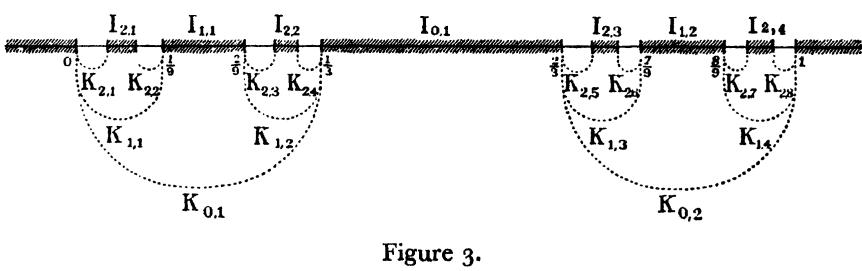
\includegraphics[keepaspectratio]{images/part002_c6c4994f.jpg}}\\
Figure 3.
If \(\mathbf{K}'\) is the complement of the union of the \(\mathbf{I}_{n,p}\) , the closed set \(\mathbf{K} = \mathbf{A} \cap \mathbf{K}'\) is called Cantor's triadic set. Clearly \(\mathbf{K}\) is compact (no. 2, Theorem 2); also \(\mathbf{K}\) is totally disconnected. For if \(\mathbf{K}\) contained an interval I of length \(>0\) , then I would be contained in some interval \(\mathbf{K}_{m,p}\) ; hence its length would be \(\leqslant 1/3^{m+1}\) for each \(m\) , which is absurd.

\subsection{HOMEOMORPHISMS OF AN INTERVAL ONTO AN INTERVAL}

THEOREM 5. Let I be an interval in R. Then a mapping f of I into R is a homeomorphism of I onto \(f(I)\) if and only if f is strictly monotonic and continuous on I; and \(f(I)\) is then an interval in R.

\begin{enumerate}
\def\labelenumi{\arabic{enumi})}
\tightlist
\item
  The condition is necessary. Let \(a\) and \(b\) be two points of \(I\) such that \(a < b\) , and suppose for example that \(f(a) < f(b)\) . Let us show that \(f\) is strictly increasing on \(I\) . First, if \(a < c < b\) then we must have \(f(a) < f(c) < f(b)\) ; if, for example, we had \(f(a) < f(b) < f(c)\)
\end{enumerate}

then the image of the interval \([a, c]\) under \(f\) would be a connected set (Chapter I, § 11, no. 2, Proposition 4) and would therefore contain the interval \([f(a), f(c)]\) ; hence there would exist \(x \in [a, c]\) such that \(f(x) = f(b)\) , contrary to the hypothesis that \(f\) is injective.

It follows that if \(x\) and \(y\) are any two points of \(I\) such that \(x < y\) , then \(f(x) < f(y)\) ; for we have \(f(a) < f(x) < f(b)\) if \(a < x < b\) , \(f(a) < f(b) < f|(x)\) if \(b < x\) , and \(f(x) < f(a) < f(b)\) if \(x < a\) ; repeating the argument with \(a, x, y\) in place of \(a, b, x\) respectively, we see that \(f(x) < f(y)\) .

\begin{enumerate}
\def\labelenumi{\arabic{enumi})}
\setcounter{enumi}{1}
\tightlist
\item
  The condition is sufficient. Suppose that \(f\) is continuous and strictly monotonic on \(I\) (say, strictly increasing): \(f(I)\) is connected and is therefore an interval, and since \(f\) is strictly increasing, \(f\) is a bijective mapping of \(I\) onto \(f(I)\) . Moreover, the image under \(f\) of an open interval in \(I\) is an open interval in \(f(I)\) , and therefore (§1, no, 4, Proposition 5) \(f\) is a homeomorphism of \(I\) onto \(f(I)\) .
\end{enumerate}

Remark. The first part of the preceding proof shows in fact that a continuous injective mapping of I into R is strictly monotonic; from the second part of the proof it therefore follows that every continuous injective mapping f of an interval I into R is a homeomorphism of I onto \(f(\mathbf{I})\) .

\section{THE FIELD OF REAL NUMBERS}

\subsection{MULTIPLICATION IN R}

The topology of the rational line \(\mathbf{Q}\) is compatible not only with the additive group structure, but also with the field structure of \(\mathbf{Q}\) . For the function \(xy\) is continuous at \((0, 0) \in \mathbf{Q} \times \mathbf{Q}\) , since for each integer \(n > 0\) the relations \(|x| \leqslant 1/n\) and \(|y| \leqslant 1/n\) together imply that \(|xy| \leqslant 1/n^2 \leqslant 1/n\) ; on the other hand, if \(a\) is any non-zero rational number, the function \(ax\) is continuous at \(x = 0\) , since for each integer \(n > 0\) the relation \(|x| \leqslant 1/n |a|\) implies that \(|ax| \leqslant 1/n\) . This shows that \(xy\) is continuous at every point of \(\mathbf{Q} \times \mathbf{Q}\) (Chapter III, § 6, no. 3).

To show that \(1 / x\) is continuous on \(\mathbf{Q}^*\) we shall establish more precisely that \(1 / x\) is uniformly continuous (with respect to the additive structure) in the complement of any neighbourhood \(\mathbf{V}\) of 0. Namely we have \(\left|\frac{1}{x} - \frac{1}{y}\right| = \frac{|x - y|}{xy}\) ; there exists an integer \(m > 0\) such that \(|x| \geqslant 1 / m\) for each \(x \in \mathbb{C}\mathbf{V}\) ; if \(x\) and \(y\) are any two points of \(\mathbb{C}\mathbf{V}\) such that \(|x - y| \leqslant 1 / m^2 n\) , we shall then have \(\left|\frac{1}{x} - \frac{1}{y}\right| \leqslant \frac{1}{n}\) .

The image, under the function \(1 / x\) , of any Cauchy filter on \(\mathbf{Q}^*\) (with respect to the additive uniformity) which does not have \(0\) as a cluster point, is a Cauchy filter (with respect to the additive uniformity). Hence (Chapter III, § 6, no. 8, Proposition 7):

PROPOSITION 1. The functions xy and 1/x, defined respectively on Q × Q and Q*, can be extended by continuity to R × R and R* respectively, and define a field structure on R. Endowed with this structure, R is called the field of real numbers.

All the properties of topological fields established in § 6 of Chapter III are of course applicable; in particular, every rational function of n real variables, with real coefficients, is continuous at every point of \(R^{n}\) where its denominator does not vanish.

\subsection{THE MULTIPLICATIVE GROUP R*}

We know from Chapter III, § 6, no. 7, that the topology induced on \(\mathbf{R}^*\) by the topology of the real line is compatible with the multiplicative group structure of \(\mathbf{R}^*\) ; since \(\mathbf{R}^*\) is an open subset of the locally compact space \(\mathbf{R}\) , it follows that \(\mathbf{R}^*\) is a locally compact topological group (Chapter I, § 9, no. 7, Proposition 13) and is therefore complete (Chapter III, § 3, no. 3, Corollary I to Proposition 4; this follows also from Chapter III, § 6, no. 8, Proposition 8); of course, this latter property relates to the multiplicative uniformity on \(\mathbf{R}^*\) and not to the uniformity induced on \(\mathbf{R}^*\) by the additive uniformity of \(\mathbf{R}\) .

The function \(xy\) maps the set \(\mathbf{Q}_{+} \times \mathbf{Q}_{+}\) into \(\mathbf{Q}_{+}\) , and therefore it maps \(\mathbf{R}_{+} \times \mathbf{R}_{+}\) into \(\mathbf{R}_{+}\) (Chapter I, § 2, no. 1, Theorem 1); in other words, the product of two real numbers \(\geqslant 0\) is \(\geqslant 0\) . The formulae \((-x)y = -xy\) and \((-x)(-y) = xy\) then show that the product of a number \(\geqslant 0\) and a number \(\leqslant 0\) is \(\leqslant 0\) , and that the product of two numbers \(\leqslant 0\) is \(\geqslant 0\) ; from this it follows that

\[
| x y | = | x |. | y |\tag{1}
\]

(which might also have been obtained by extension of the corresponding relation on \(\mathbf{Q} \times \mathbf{Q}\) ).

If \(x > 0\) and \(y > 0\) we have \(xy \neq 0\) , and therefore \(xy > 0\) ; likewise, if \(x < 0\) and \(y > 0\) , then \(xy < 0\) ; and if \(x < 0\) and \(y < 0\) , then \(xy > 0\) . In particular, if \(x \neq 0\) we have \(x^2 > 0\) , so that a sum of squares of real numbers cannot be zero unless each of the numbers is zero.

If \(x > 0\) and \(y \leqslant z\) (resp. \(y < z\) ) we have \(xy \leqslant xz\) (resp. \(xy < xz\) ) in other words, a homothety of ratio \(> 0\) preserves order on \(\mathbf{R}\) . Since \((-x)y = -xy\) , a homothety of ratio \(< 0\) changes the ordering on \(\mathbf{R}\) into the opposite ordering.

If \(x > 0\) we have \(\mathbf{1} / x > 0\) , since \(x.(\mathbf{1} / x) = \mathbf{1} > 0\) . If \(0 < x < y\) we have \(xy > 0\) , hence \(x.(\mathbf{1} / xy) < y.(\mathbf{1} / xy)\) , that is \(\mathbf{1} / y < \mathbf{1} / x\) . Hence the mapping \(x \to \mathbf{1} / x\) of the set \(\mathbb{R}_+^*\) of real numbers \(> 0\) onto itself is strictly decreasing.

We see in the same way that the function \(\mathbf{1} / x\) is strictly decreasing in \(] \leftarrow, o[, \text{ and therefore the function } \frac{\mathbf{1}}{x - a}\) is strictly decreasing in each of the intervals \(] \leftarrow, a[ \text{ and } ]a, \rightarrow [.\)

It follows from what precedes that \(R_{+}^{*}\) is a subgroup of the multiplicative group \(R^{*}\) ; moreover, the order relation \(x \leqslant y\) is compatible with the multiplicative, group structure of \(R_{+}^{*}\) ; in other words, \(R_{+}^{*}\) is a linearly ordered group.

The fact that the product of two real numbers \(\geqslant0\) is \(\geqslant0\) can be expressed by saying that R is an ordered field: all the above properties are common to all ordered fields.

PROPOSITION 2. The multiplicative group \(\mathbf{R}^{*}\) of real numbers \(\neq 0\) is a topological group isomorphic to the product of its subgroups \(\mathbf{R}_{+}^{*}\) and \(\mathbf{U}_{0}\) , where

\[
\mathrm{U} _ {0} = \{- 1, + 1 \}.
\]

For each \(x \neq 0\) let \(\operatorname{sgn} x\) denote \(\frac{x}{|x|}\) (sign of \(x\) ). The function \(\operatorname{sgn}\) is a homomorphism of \(\mathbf{R}^*\) onto \(U_0\) . We have \(x = |x| \operatorname{sgn} x\) , and this decomposition of \(x\) as the product of an element of \(\mathbf{R}_+^*\) and an element of \(U_0\) is unique; hence the group structure of \(\mathbf{R}^*\) is the product of the group structures of \(\mathbf{R}_+^*\) and \(U_0\) . On the other hand, the mapping \(x \to |x|\) is continuous, and so is \(x \to \operatorname{sgn} x = \frac{x}{|x|}\) , since \(x \neq 0\) . Hence the result.

We extend the function sgn to the whole of R by putting sgn o = o.

We shall see in Chapter V (§ 4, no. 1, Theorem 1) that the topological group \(\mathbf{R}_{+}^{*}\) is isomorphic to the additive group \(\mathbf{R}\) ; this will complete the determination of the structure of the topological group \(\mathbf{R}^{*}\) .

\subsection{nTH ROOTS}

Let \(n\) be any integer \(> 0\) . From the relation \(0 < x < y\) we deduce, by induction on \(n\) , that \(0 < x^n < y^n\) . In other words, the function \(x \to x^n\) is strictly increasing for \(x \geqslant 0\) ; it is clearly continuous at every point and therefore (§ 2, no. 6, Theorem 5) it is a homeomorphism of \(\mathbf{R}_{+}\) onto an interval \(\mathbf{I}\) . On the other hand, since \(x \geqslant 1\) implies \(x^{n-1} \geqslant 1\) and therefore \(x^n \geqslant x\) , it follows that \(\mathbf{I}\) is not bounded and hence \(\mathbf{I} = \mathbf{R}_{+}\) . The value, for \(x \geqslant 0\) , of the inverse of the mapping \(x \to x^n\) is denoted by \(x^{1/n}\) or \(\sqrt[n]{x}\) and is called \(x\) to the power \(1\) or the nth root of \(x\) (for \(n = 2\) , 3 we say square root, cube root; for \(n = 2\) we write \(\sqrt{x}\) in place of \(\sqrt[2]{x}\) ). The positive number \(x^{1/n}\) is thus defined as the unique positive solution of the equation

\[
y ^ {n} = x \quad (x \geqslant 0).\tag{2}
\]

In particular we see that there is a real number x such that \(x^{2}=2\) , whereas no rational number has this property; thus we recover the fact that the rational line Q is not a complete space.

The mapping \(x \to x^{1/n}\) of \(\mathbf{R}_+\) onto itself is strictly increasing and continuous. By (2) we have \(0^{1/n}=0, 1^{1/n}=1\) , also

\[
(x y) ^ {1 / n} = x ^ {1 / n} y ^ {1 / n};\tag{3}
\]

hence \(x \to x^{1/n}\) is an automorphism of the topological group \(\mathbf{R}_{+}^{*}\) .

In Chapter V, § 4, no. 1, we shall generalize this result by finding all the automorphisms of the multiplicative group \(\mathbf{R}_{+}^{*}\) .

\section{THE EXTENDED REAL LINE}

\subsection{HOMEOMORPHISMS OF OPEN INTERVALS OF R}

PROPOSITION 1. All non-empty open intervals of \(\mathbf{R}\) are homeomorphic to \(\mathbf{R}\) . Consider first a bounded open interval \(\mathbf{I} = ]a\) , \(b[(a < b)\) . For each \(x \in \mathbf{I}\) put \(f(x) = -\left(\frac{1}{x - a} + \frac{1}{x - b}\right)\) . This function is continuous and strictly increasing on \(\mathbf{I}\) , for we have seen that \(\frac{1}{x - b}\) is strictly decreasing in \(]\leftarrow, b[\) and \(\frac{1}{x - a}\) strictly decreasing in \(]a, \rightarrow[\) . It follows that \(f\) is a homeomorphism of \(\mathbf{I}\) onto an interval \(f(\mathbf{I})\) of \(\mathbf{R}\) ( \(\S 2\) , no. 6, Theorem 5). \(f(\mathbf{I})\) is neither bounded above nor below; if, for example, we had \(f(x) \leqslant c\) for all \(x \in \mathbf{I}\) , it would follow that \(1 - \frac{b - x}{x - a} \leqslant c(b - x)\) , since \(b - x > 0\) ; and this leads to a contradiction when \(x\) is sufficiently near \(b\) (by virtue of the continuity of the two sides of the inequality, which are rational functions, at the point \(b\) ). Hence \(f(\mathbf{I}) = \mathbf{R}\) , and therefore every bounded open interval is homeomorphic to \(\mathbf{R}\) . Let \(g\) be the inverse of \(f\) : it maps every unbounded open interval of \(\mathbf{R}\) onto an interval \(J\) contained in \(I\) and open in \(I\) . Since \(I\) is open in \(\mathbf{R}\) , \(J\) is also open in \(\mathbf{R}\) ; since it is bounded, it is homeomorphic to \(\mathbf{R}\) ; and thus we have proved that every unbounded open interval is homeomorphic to \(\mathbf{R}\) .

Remark. To show that all bounded open intervals are homeomorphic to each other, it would be enough to remark that, if \(a \neq b\) and \(a' \neq b'\) , there is a homeomorphism of R onto itself, of the form \(x \to \alpha x + \beta\) (and only one) which maps a to \(a'\) and b to \(b'\) , and hence maps the open (resp. half-open, closed) interval with end-points a, b onto the open (resp. half-open, closed) interval with end-points \(a', b'\) ; the reader may easily verify this by calculating \(\alpha\) and \(\beta\) .

\subsection{THE EXTENDED LINE}

We shall now define, by adjoining two new elements to R, a topological space \(\overline{R}\) such that every homeomorphism of R onto a bounded open interval I of R can be extended to a homeomorphism of \(\overline{R}\) onto the closed interval having the same end-points as I.

Let \(\overline{\mathbf{R}}\) be the set obtained by adjoining (Set Theory, R, § 4, no. 5) two new elements to \(\mathbf{R}\) , denoted by \(-\infty\) and \(+\infty\) . We extend the ordering on \(\mathbf{R}\) to \(\overline{\mathbf{R}}\) by putting \(-\infty < a\) and \(a < +\infty\) for all \(a \in \mathbf{R}\) , and \(-\infty < +\infty\) ; it is clear that we thus obtain a linearly ordered set, whose ordering induces the ordering of the real line on \(\mathbf{R}\) . Next, consider the topology on \(\overline{\mathbf{R}}\) generated by the set of open intervals of \(\overline{\mathbf{R}}\) . Since the trace on \(\mathbf{R}\) of an open interval of \(\overline{\mathbf{R}}\) is an open interval of \(\mathbf{R}\) , this topology induces on \(\mathbf{R}\) the topology of the real line.

DEFINITION 1. The set \(\overline{\mathbf{R}}\) endowed with the order structure and the topology defined above is called the extended real line.

When using the extended line \(\overline{\mathbf{R}}\) it is often convenient to refer to its points as real numbers, by abuse of language; the points of \(\mathbf{R}\) are then called finite real numbers. We shall adopt this convention in this section and the three following sections of this chapter; whenever we adopt this convention in future we shall indicate explicitly to which part of the text it extends.

If \(a\) is a finite real number, the intervals \([a, +\infty[ \text{ and } ] - \infty, a]\) (resp. \(]a, +\infty[ \text{ and } ] - \infty, a[\) ) of \(\overline{\mathbf{R}}\) are contained in \(\mathbf{R}\) and coincide with the intervals of \(\mathbf{R}\) hitherto denoted by \([a, \rightarrow[ \text{ and } ] \leftarrow, a]\) (resp. \(]a, \rightarrow[ \text{ and } ] \leftarrow, a[\) ); this new notation is much more often used. Again, \(\mathbf{R}\) coincides with the interval \(] - \infty, +\infty[ \text{ of } \overline{\mathbf{R}}, \text{ and is sometimes so denoted.}\)

PROPOSITION 2. Every homeomorphism \(f\) of \(\mathbf{R}\) onto an interval \(]a, b[\) can be extended to a homeomorphism \(\overline{f}\) of \(\overline{\mathbf{R}}\) onto \([a, b]\) . If \(f\) is an increasing function, then \(\overline{f}\) is an order isomorphism of \(\overline{\mathbf{R}}\) onto \([a, b]\) .

Let \(f\) be an increasing homeomorphism. If we extend \(f\) to \(\mathbf{R}\) by putting \(\overline{f}(-\infty) = a\) and \(\overline{f}(+\infty) = b\) , it is obvious that \(\overline{f}\) is a strictly increasing mapping (and therefore a bijection) of \(\overline{\mathbf{R}}\) onto \([a, b]\) . Hence \(\overline{f}\) maps every open interval of \(\overline{\mathbf{R}}\) onto an interval which is open with respect to \([a, b]\) , and is therefore a homeomorphism of \(\overline{\mathbf{R}}\) onto \([a, b]\) by reason of Definition 1 and Proposition 5 of § 1, no. 4.

If \(f\) is decreasing, we apply what has been proved to the increasing homeomorphism \(x \to -f(x)\) of \(\mathbf{R}\) onto \(] - b, - a[\) .

All the properties of the interval \([a, b]\) obtained in §2, which involve only the order structure and the topology of the interval, can therefore be transported to \(\overline{R}\) ; hence the following propositions:

PROPOSITION 3. The extended real line is compact.

Hence (Chapter II, § 4, no. 1, Theorem 1) there is a unique uniformity on \(\overline{\mathbf{R}}\) compatible with its topology; this uniformity is isomorphic with the uniformity induced on \([a, b]\) by the additive uniformity of \(\mathbf{R}\) . But it should be remarked that the uniformity induced on \(\mathbf{R}\) by that of \(\overline{\mathbf{R}}\) is not the additive uniformity of \(\mathbf{R}\) (although it is compatible with the topology of the real line); for \(\mathbf{R}\) is a complete space with respect to its additive uniformity, but is not a complete subspace of \(\overline{\mathbf{R}}\) , since it is not closed in \(\overline{\mathbf{R}}\) .

PROPOSITION 4. Every non-empty subset of \(\overline{\mathbf{R}}\) has a least upper bound and a greatest lower bound.

The least upper bound (resp. greatest lower bound) of a non-empty subset A of R is denoted by sup A (resp. inf A). Clearly

\[
\inf A \leqslant \sup A.\tag{1}
\]

If \(\mathbf{A} \subset \mathbf{B}\) , then \(\sup \mathbf{A} \leqslant \sup \mathbf{B}\) and \(\inf \mathbf{A} \geqslant \inf \mathbf{B}\) (Set Theory, Chapter III, § 1, no. 9, Proposition 4).

PROPOSITION 5. A subset A of \(\overline{R}\) is connected if and only if A is an interval.

COROLLARY. The extended real line is a connected, locally connected space.

PROPOSITION 6. A mapping \(f\) of an interval \(I\) of \(\overline{R}\) into \(\overline{R}\) is a homeomorphism of \(I\) onto \(f(I)\) if and only if \(f\) is strictly monotonic and continuous on \(I\) ; \(f(I)\) is then an interval of \(\overline{R}\) .

Finally, the functions \(\sup (x,y)\) and \(\inf (x,y)\) are continuous on \(\overline{\mathbf{R}}\times \overline{\mathbf{R}}\)

\subsection{\texorpdfstring{ADDITION AND MULTIPLICATION IN \(\bar{R}\)}{ADDITION AND MULTIPLICATION IN \textbackslash bar\{R\}}}

Note first that the function \(-x\) can be extended by continuity to \(\overline{\mathbf{R}}\) , according to the formulae \(-(-\infty)=+\infty\) and \(-(+\infty)=-\infty\) ; the function thus extended is a homeomorphism of \(\overline{\mathbf{R}}\) onto itself.

Next, consider, the functions \(x + y\) and xy, defined on \(R \times R\) , with values in R; by considering that they take their values in the topological space \(\overline{R}\) , we shall see that they too can be extended by continuity at certain points of \(\overline{R} \times \overline{R}\) .

So far as \(x + y\) is concerned, let \(A' = ] - \infty, + \infty]\) and \(A'' = [-\infty, + \infty[\) . Then we have the following proposition:

PROPOSITION 7. The function \(x + y\) can be extended by continuity to each of the sets \(\mathbf{A}' \times \mathbf{A}'\) and \(\mathbf{A}'' \times \mathbf{A}''\) , according to the formulae

\[
\left\{ \begin{array}{l l} x + (+ \infty) = (+ \infty) + x = + \infty & (x \neq - \infty), \\ x + (- \infty) = (- \infty) + x = - \infty & (x \neq + \infty). \end{array} \right.\tag{2}
\]

Let us show, for example, that as \((x,y)\) tends to the point \((a,+\infty)\) \((a\neq-\infty)\) while remaining in \(R\times R\) , \(x+y\) tends to \(+\infty\) . There exists a finite number b\textless a, and the interval {]}b, \(+\infty\) {[} is a neighbourhood of a in R; given any finite c, the relations x\textgreater b and y\textgreater c-b imply \(x+y>c\) , and this shows that \(x+y\) is as near as we please to \(+\infty\) whenever \((x,y)\) is near enough to \((a,+\infty)\) . The argument is similar in the other cases.

On the contrary, \(x + y\) has no limit at the points \((-\infty, +\infty)\) and \((+\infty, -\infty)\) of \(\overline{\mathbf{R}} \times \overline{\mathbf{R}}\) . For if \(x + y\) had limit \(k\) (finite or infinite) as \((x, y)\) tends to \((+\infty, -\infty)\) while remaining in \(\mathbf{R} \times \mathbf{R}\) , it would follow that, for each finite \(a\) , the function \((x + a) - x\) would tend to \(k\) as \(x\) tends to \(+\infty\) while remaining in \(\mathbf{R}\) ; and this is absurd, since \((x + a) - x = a\) and \(a\) is arbitrary.

The function \(x + y\) maps \(A' \times A'\) (resp. \(A'' \times A''\) ) into \(A'\) (resp. \(A''\) ). It is therefore a law of composition on \(A'\) (resp. \(A''\) ) which extends the law of addition on \(R\) . By the principle of extension of identities (Chapter I, § 8, no. 1, Corollary 1 to Proposition 2) this law is commutative and associative; o is the identity element for this law; and the only non-regular element (Algebra, Chapter I, § 2, no. 2) of \(A'\) is \(+\infty\) , by formulae (2).

If \(x, y, z, t\) are points of \(\overline{\mathbf{R}}\) such that \(x \leqslant y\) and \(z \leqslant t\) , then \(x + z \leqslant y + t\) whenever both sides of this inequality are defined.

Note that in \(\overline{\mathbf{R}}\) the relation \(x < y\) implies \(x + z < y + z\) only if \(z\) is finite, by formulae (2); it is easily verified that the relations \(x < y\) and \(z < t\) imply \(x + z < y + t\) whenever both sides of this inequality are defined.

In \(\overline{\mathbf{R}}\) we put \(x^{+} = \sup (x,0)\) , \(x^{-} = \sup (-x,0)\) , \(|x| = \sup (x, - x)\) ; thus \((+\infty)^{+} = (-\infty)^{-} = +\infty\) and \((+\infty)^{-} = (-\infty)^{+} = 0\) , and \(|+\infty| = |- \infty| = +\infty\) . The sums \(x^{+} - x^{-}\) and \(x^{+} + x^{-}\) are defined for all \(x \in \overline{\mathbf{R}}\) and are therefore equal to \(x\) and \(|x|\) respectively by the principle of extension of identities. Also, whenever the sum \(x + y\) is defined, we have \(|x + y| \leqslant |x| + |y|\) .

Note on the contrary that formulae (6) and (7) of § 1, no. 1 may no longer make sense for certain values of \(x\) and \(y\) in \(\overline{\mathbf{R}}\) ; for example, if \(x = -\infty\) and \(y = 0\) we have \(\sup (x, y) = 0\) , but the sum \(x + (y - x)^+\) is not defined, because \((y - x)^+ = +\infty\) .

Let \(\overline{\mathbf{R}}^{*}\) denote the complement of \(o\) in \(\overline{\mathbf{R}}\) . Then the analogue of Proposition 7 for multiplication runs as follows:

PROPOSITION 8. The function \(xy\) can be extended by continuity to the set \(\overline{\mathbf{R}}^* \times \overline{\mathbf{R}}^*\) according to the formulae

\[
\left\{ \begin{array}{l} x. (+ \infty) = (+ \infty). x = \left\{ \begin{array}{l l} + \infty & \text {if} \quad x > 0 \\ - \infty & \text {if} \quad x <   0 \end{array} \right. \\ x. (- \infty) = (- \infty). x = \left\{ \begin{array}{l l} - \infty & \text {if} \quad x > 0 \\ + \infty & \text {if} \quad x <   0. \end{array} \right. \end{array} \right.\tag{3}
\]

We leave the proof to the reader; it is analogous to the proof of Proposition 7.

Likewise, we see that \(xy\) has no limit at the points \((0, +\infty), (+\infty, 0), (0, -\infty), (-\infty, 0)\) of \(\overline{\mathbf{R}} \times \overline{\mathbf{R}}\) .

The function \(xy\) is a law of composition on \(\overline{\mathbf{R}}^*\) which extends the law of multiplication on \(\mathbf{R}\) ; this law is associative and commutative (principle of extension of identities); it has 1 as identity element; and the non-regular elements in \(\overline{\mathbf{R}}^*\) are \(+\infty\) and \(-\infty\) .

If \(x \leqslant y\) and \(z > 0\) we have \(xz \leqslant yz\) whenever both sides of this inequality are defined. If the product \(xy\) is defined, then so is \(|x| \cdot |y|\) and we have \(|xy| = |x| \cdot |y|\) .

Finally, the distributivity formula

\[
x (y + z) = x y + x z\tag{4}
\]

is still valid, by virtue of the principle of extension of identities, whenever all the operations which figure on either side are defined.

\pandocbounded{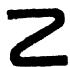
\includegraphics[keepaspectratio]{images/part002_cca5eabe.jpg}}

Note that it can happen that the left-hand side of (4) is defined while the right-hand side is not: for example, consider the case where \(x = +\infty\) , y = 2 and z = -1. The distributivity formula should therefore be used with caution in R.

\section{REAL-VALUED FUNCTIONS}

\subsection{REAL-VALUED FUNCTIONS}

DEFINITION 1. A mapping of a set X into the real line is called a real-valued function (or real function) defined on X.

By an abuse of language analogous to that mentioned in § 4, no. 2, mappings of X into \(\overline{\mathbf{R}}\) will also be called real-valued functions defined on X in this and the following section. Mappings of X into \(\mathbf{R}\) will be called finite real-valued functions.

If \(f\) and \(g\) are two real-valued functions defined on \(\mathbf{X}\) , the relation \(f \leqslant g\) is by definition equivalent to `` \(f(x) \leqslant g(x)\) for all \(x \in \mathbf{X}\) ;'' this relation is an ordering on the set \(\overline{\mathbf{R}}^{\mathbf{X}}\) of all real-valued functions on \(\mathbf{X}\) . The set \(\overline{\mathbf{R}}^{\mathbf{X}}\) ordered by this relation, is a lattice; for if \(f\) and \(g\) are any two real-valued functions, the function \(h\) defined by \(h(x) = \sup (f(x), g(x))\) for all \(x \in \mathbf{X}\) is the smallest of the real-valued functions on \(\mathbf{X}\) which are both \(\geqslant f\) and \(\geqslant g\) ; in accordance with general notation, we denote this function (which is the least upper bound of \(f\) and \(g\) in \(\overline{\mathbf{R}}^{\mathbf{X}}\) ) by \(\sup (f, g)\) . Similarly, the function whose value at each \(x \in \mathbf{X}\) is \(\inf (f(x), g(x))\) is denoted by \(\inf (f, g)\) .

Note that sup \((f, g)\) is the composition of the mapping

\[
(u, v) \mapsto \sup (u, v)
\]

of \(\overline{\mathbf{R}}\times \overline{\mathbf{R}}\) into \(\overline{\mathbf{R}}\) and the mapping \(x\to (f(x),g(x))\) of \(\mathbf{X}\) into \(\overline{\mathbf{R}}\times \overline{\mathbf{R}}\) . Similarly for inf \((f,g)\) .

A real-valued function \(f\) defined on a set \(\mathbf{X}\) is said to be bounded above (resp. bounded below) in \(\mathbf{X}\) , if \(f(\mathbf{X})\) is a subset of \(\mathbf{A}'' = [-\infty, +\infty[\) and is bounded above (resp. if \(f(\mathbf{X})\) is a subset of \(\mathbf{A}' = ] - \infty, +\infty]\) and is bounded below). \(f\) is said to be bounded in \(\mathbf{X}\) if it is bounded both above and below, that is if \(f(\mathbf{X})\) is a bounded subset of \(\mathbf{R}\) .

Every bounded function is therefore finite. The converse is false, as is shown by the function \(\mathbf{1} / x\) on \(\mathbb{R}_+^* = ]0, +\infty[\) .
